\chapter{路面驾驶机器人单目视觉里程计简化}
% Problem

人类的日常生活越来越多地涉及到移动机器人,包括自主地面车辆(AGV)、无人驾驶飞行器(UAV)和服务机器人。
移动机器人在复杂的环境中进行导航和执行任务时,必须对自己进行定位。
在环境未开发的情况下,既没有全球定位系统(GPS),也没有环境地图,无法进行绝对状态估计,只能采取相对状态估计,又称为增量式定位方法,如视觉测距。
该方法是通过累积式增量计算机器人相对于到它的起始坐标系中的增量自我运动(包括平移和旋转运动),与构建的地图无关。
大多数VO利用基于几何学的方法来估计自我运动$(\mathbf{R},\mathbf{t})$,
通过最小化重投影误差\cite{raul2015orb}(基于特征的方法)或最小化光学误差\cite{Engel-et-al-pami2018}(直接法)。
然而,这些方法需要准确的传感器校准和手动参数调整,以便在不同的环境中良好地工作\cite{roberts2008memory}。
但是,参数调整过程需要工程师根据状态反馈不断进行调整,是一项消耗精神与时间的繁琐工作。


为了减少人为调整参数的努力,很多研究工作都投入到基于学习的端到端方法中。
用基于学习的方法进行自我运动估计是由Roberts等人开始的\cite{roberts2008memory},他们尝试用K-Nearest Neighbors模型学习从光流到二维运动的映射。 
其他许多开创性的方法也在探索建立从光流到小我运动的映射模型\cite{guizilini2012semi,costante2016exploring,pillai2017towards,costante2018ls}。
Wang等人\cite{wang2017deepvo,wang2018end}首先提出了从原始图像到自我运动的端到端模型。除此之外,Wang等人还通过使用递归神经网络来处理图像序列信息。
为了减少标签数据的依赖性,Zhou等人/\cite{zhou2017unsupervised}提出了两个无监督的网络结构,与图像深度预测与自我运动估计相结合,将重投影图像的残差作为损失函数。
在此基础上,许多研究人员设计了不同损失函数进行网络改进:增加额外的3D几何损失函数\cite{mahjourian2018unsupervised},双目损失函数\cite{li2018undeepvo},深度特征重建损失函数\cite{zhan2018unsupervised},动态和光流损失函数\cite{yin2018geonet}或相对损失函数\cite{almalioglu2019ganvo}来等。
为了实现系统的鲁棒性,Klodt等人\cite{klodt2018supervising}和Yang等人\cite{yang2020d3vo}进一步提出测评自我运动和深度的不确定性。而Clement等人\cite{clement2018train}则试图用图像转换模型来增加算法对光照的鲁棒性。


H然而,基于端到端深度学习方法的表现仍然不容乐观。我们发现其中一个基本问题是基于学习的方法总是依赖于一个庞大而多样化的数据集来训练一个性能良好的模型。如Imagenet数据集\cite{deng2009imagenet}用于物体检测,Cityscape数据集\cite{Cordts2016Cityscapes}用于语义分割。然而,对于地面车辆的自我运动估计,
最显著的数据集如KITTI\cite{geiger2012kitti}和Robotcar\cite{RobotCarDatasetIJRR},而用于移动机器人视觉定位的开源训练数据集在图片数量和多样性上仍十分有限。
Zhou等人的自监督方法\cite{zhou2017unsupervised}可以减弱对地面车辆运动ground truth的依赖性,降低了训练数据采集难度,但他们并没有解决对训练数据数量的要求,因为他们仍然依赖于图像序列。
为了应对训练数据集的局限性,Slinko等人\cite{slinko2019training}提出基于RGB-D图像的随机重投影来生成训练集,增加的训练数据的可利用性。
此外,Wang等人\cite{wang2020tartanair}通过模拟不同的环境和具有挑战性的光照条件,收集了一个更大的具有复杂运动模式的数据集。


为了降低网络对数据集的依赖,我们提出通过简化学习目标,在有限的KITTI数据集上学习视觉里程计深度模型。

我们观察发现,以往的路面机器人在实现自我定位时,学习的是六自由度的运动$\textbf{R}$和$\textbf{t}$。然而,在车辆的行驶过程中,其主要运动(如图\ref{fig:car_simplify}所示)。由于地面车辆的运动受到其机械结构和动力学的限制,所以如果我们的深度网络结构只专注于主要运动时并不会导致过多的姿势偏移。
另外,我们观察发现由于噪声的存在,观察到的次要运动总是具有较低的信噪比。基于以上观察我们得出结论,当深度学习网络聚焦于学习地面车辆的
主要运动时,可以减少对训练数据量的依赖,简化学习问题的同时可以降低其余自由度带来的冗余误差,是一个可观的深度学习视觉定位方案。

地面车辆的约束运动模型已被广泛采用在基于几何学的视觉里程测量方法中。%许多方法都是利用安装摄像头的固定高度作为绝对参考来恢复单目视觉里程计的尺度。
Scaramuzza等人\cite{scaramuzza2009real}基于运动约束和阿克曼转向定律\cite{siegwart2011introduction}提出1-point-RANSAC用于自我动作估计,
以提高实时性能。Choi等人\cite{choi2015simplified}考虑了突然的颠簸或相机振动,并放宽了平面假设。Scaramuzza等人 \cite{4625958}利用全向相机提
供的地面特征点根据单应性矩阵法计算机器人自我运动位姿。

\begin{figure}[h]
    \centering
    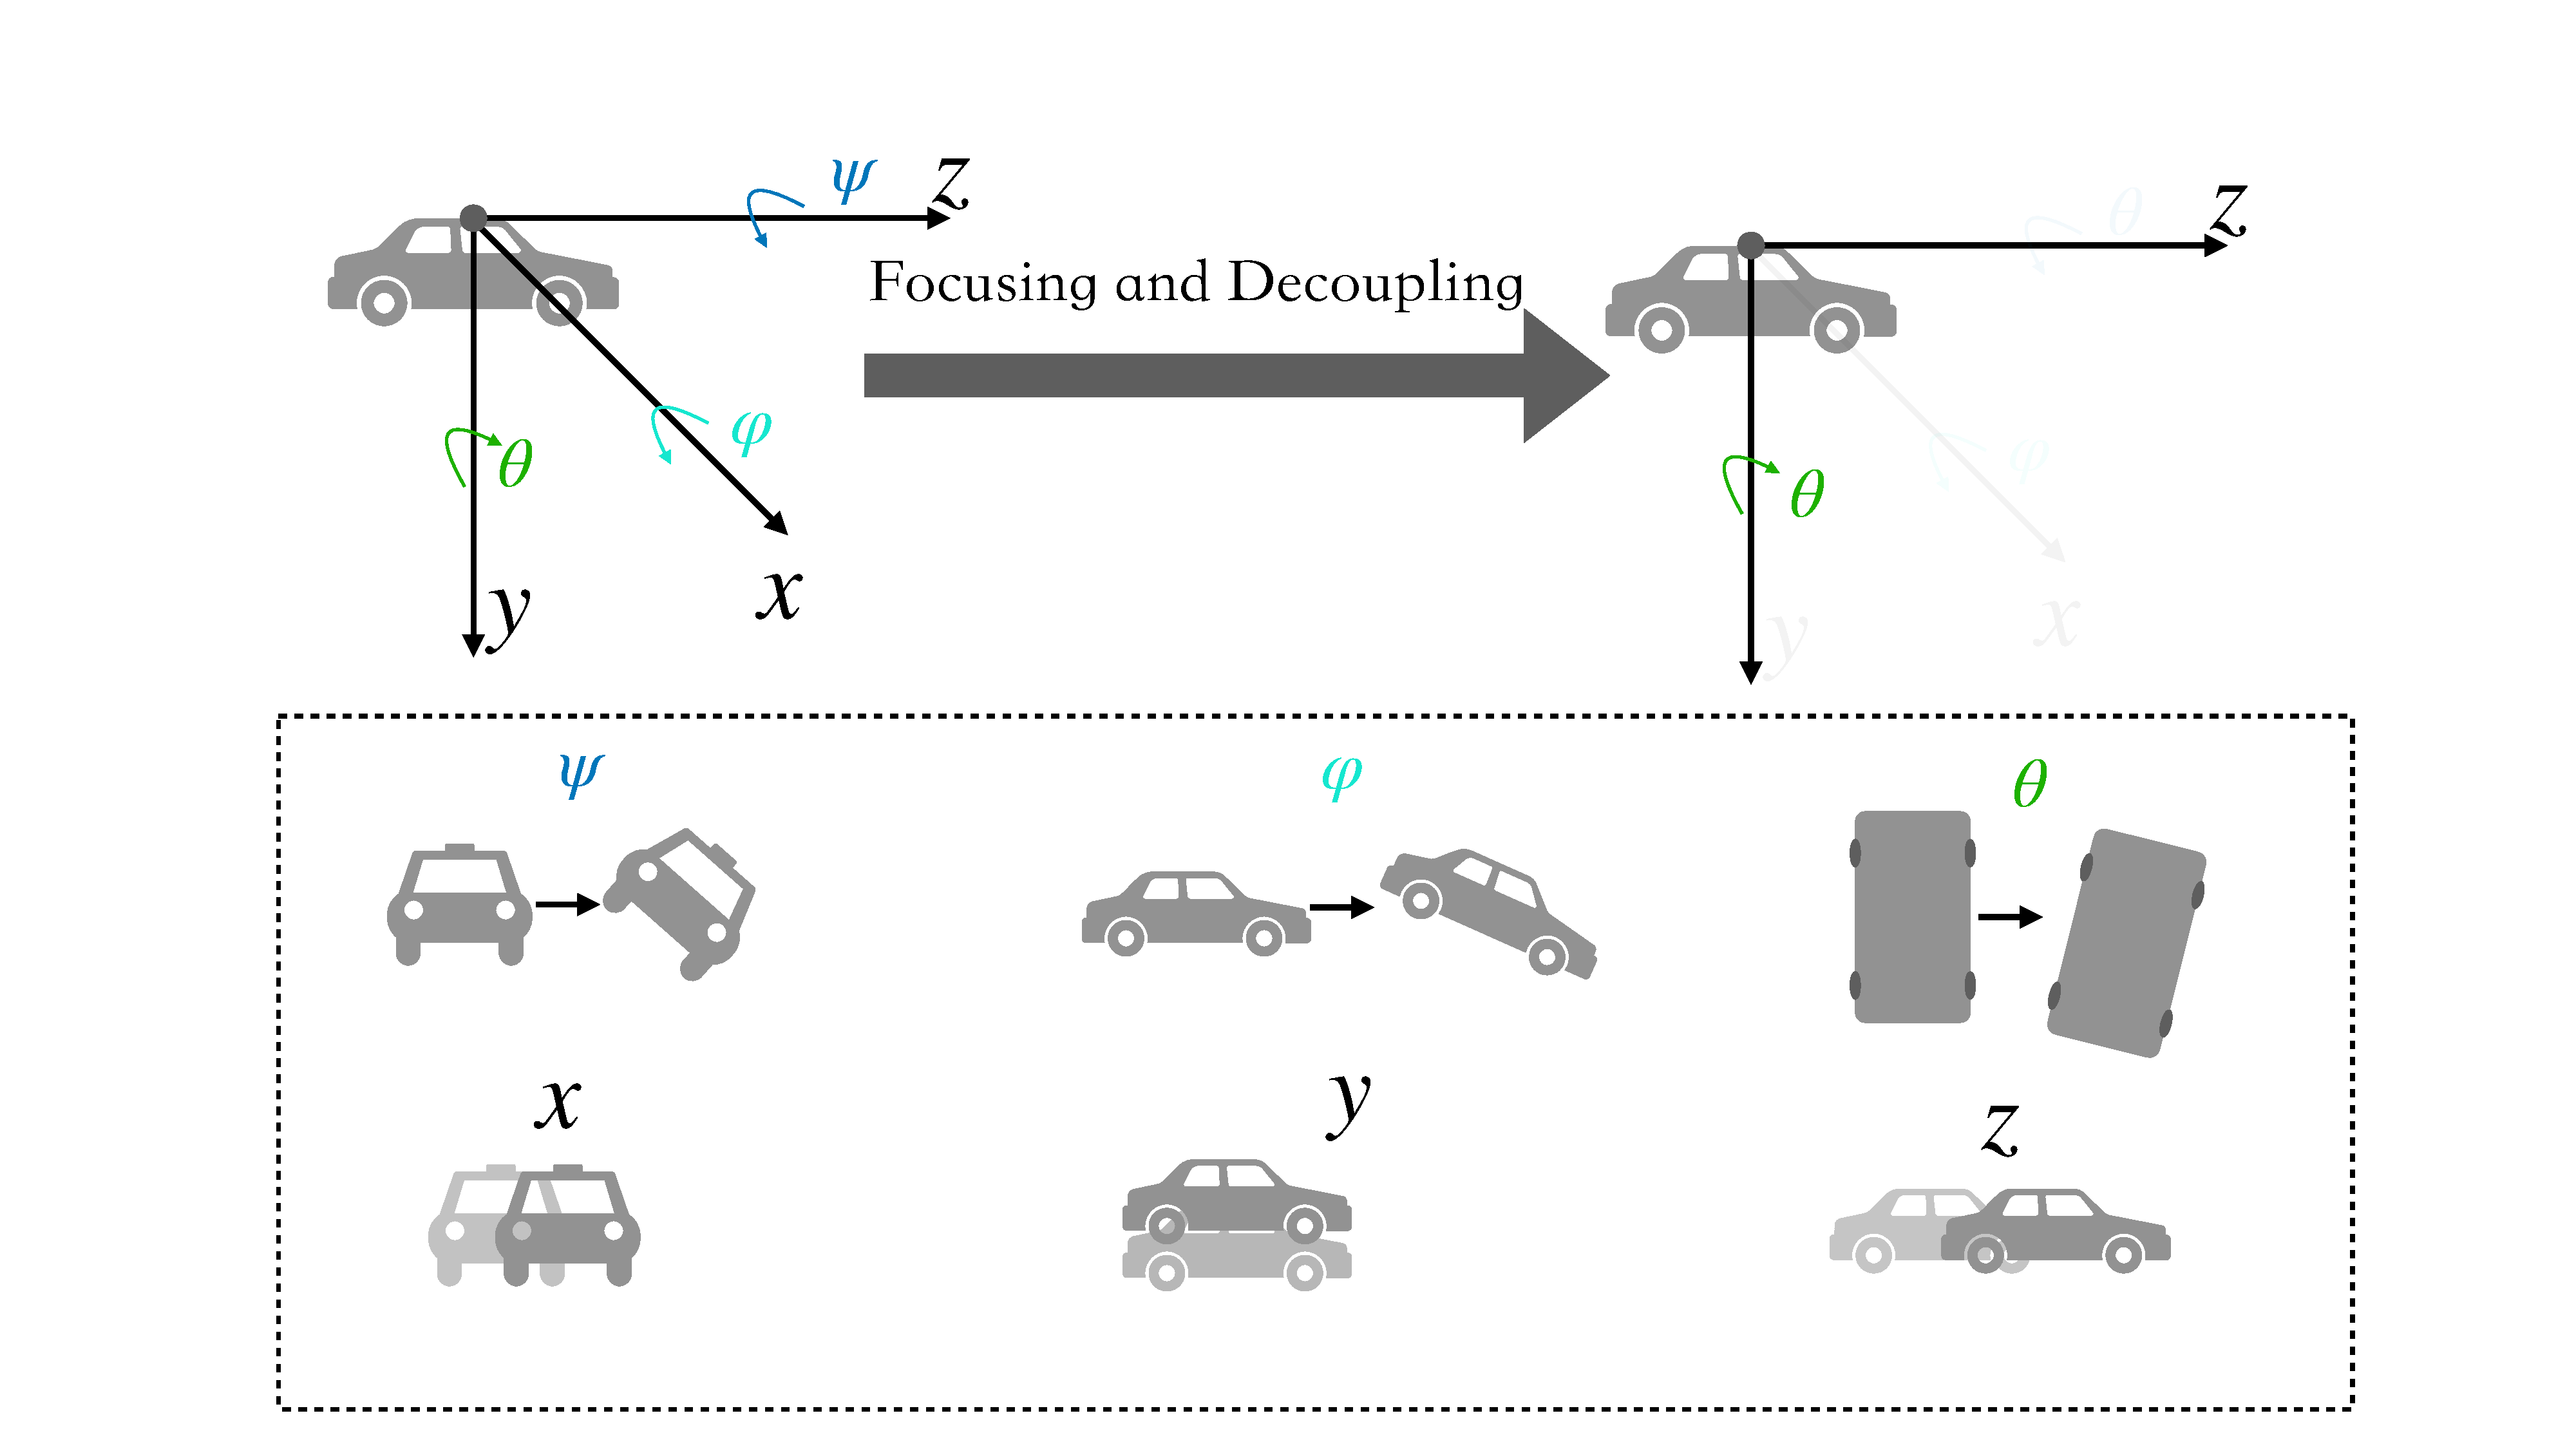
\includegraphics[width=0.7\textwidth]{datavo/car_simplify.pdf}
    \caption{动机:将网络学习目标集中在路面车辆的主要运动上以简化深度学习目标并降低冗余误差。}
    \label{fig:car_simplify}
\end{figure}

本文尝试了一种全新的路面车辆运动模型,我们将神经网络的学习目标集中在主要运动的自由度上(命名为运动聚焦),并定量评估了当忽略某个次要运动自由度时所引起的姿态位移,
并探讨了通过考虑地面车辆运动模型(命名为运动解耦)来最小化姿态位移。

此外,我们构建了仅有4个卷积层的轻型卷积神经网络来学习地面车辆的显著运动,并进行了实验,表明运动聚焦与运动解耦可以提高自我运动估计性能。整个系统的结构如图所示\ref{fig:system_structure}。本章的主要贡献是:

\begin{enumerate}
    \item {通过对运动聚焦引起的地面真实姿势位移进行定量评估,发现其位移相对较小,可以通过实验证明运动聚焦的可行性;}
    \item {分析了X轴意外平移的原因,建立了X轴平移和Y轴旋转的关系模型,并利用该模型来减少运动解耦引起的姿势位移;}
    \item {我们在KITTI数据集上进行了对比实验,表明所提出的运动聚焦和解耦可以减少训练时间,提高学习性能;}
    \item {构建了轻型卷积神经网络来模拟地面车辆的主要运动,模型足够轻,可以在GPU上用2G左右的内存进行训练,并在CPU上实时运行(每秒超过200帧)。
    为了促进视觉里程计的发展,我们公开了源代码\footnote{https://github.com/TimingSpace/DMVOGV}。}
\end{enumerate}

本文的其余部分组织如下。第一节\ref{sec:IEEEAccess_approach}描述了我们的方法,包括运动聚焦和训练细节。在第\ref{sec:IEEEAccess_experiments}节中,我们的方法在KITTI数据集\cite{geiger2012kitti}上进行了评估。我们在\ref{sec:IEEEAccess_conclusion}中对本文进行了总结并讨论了未来的工作。
\section{方法}
\label{sec:IEEEAccess_approach}

\begin{figure*}[t]
    \centering
    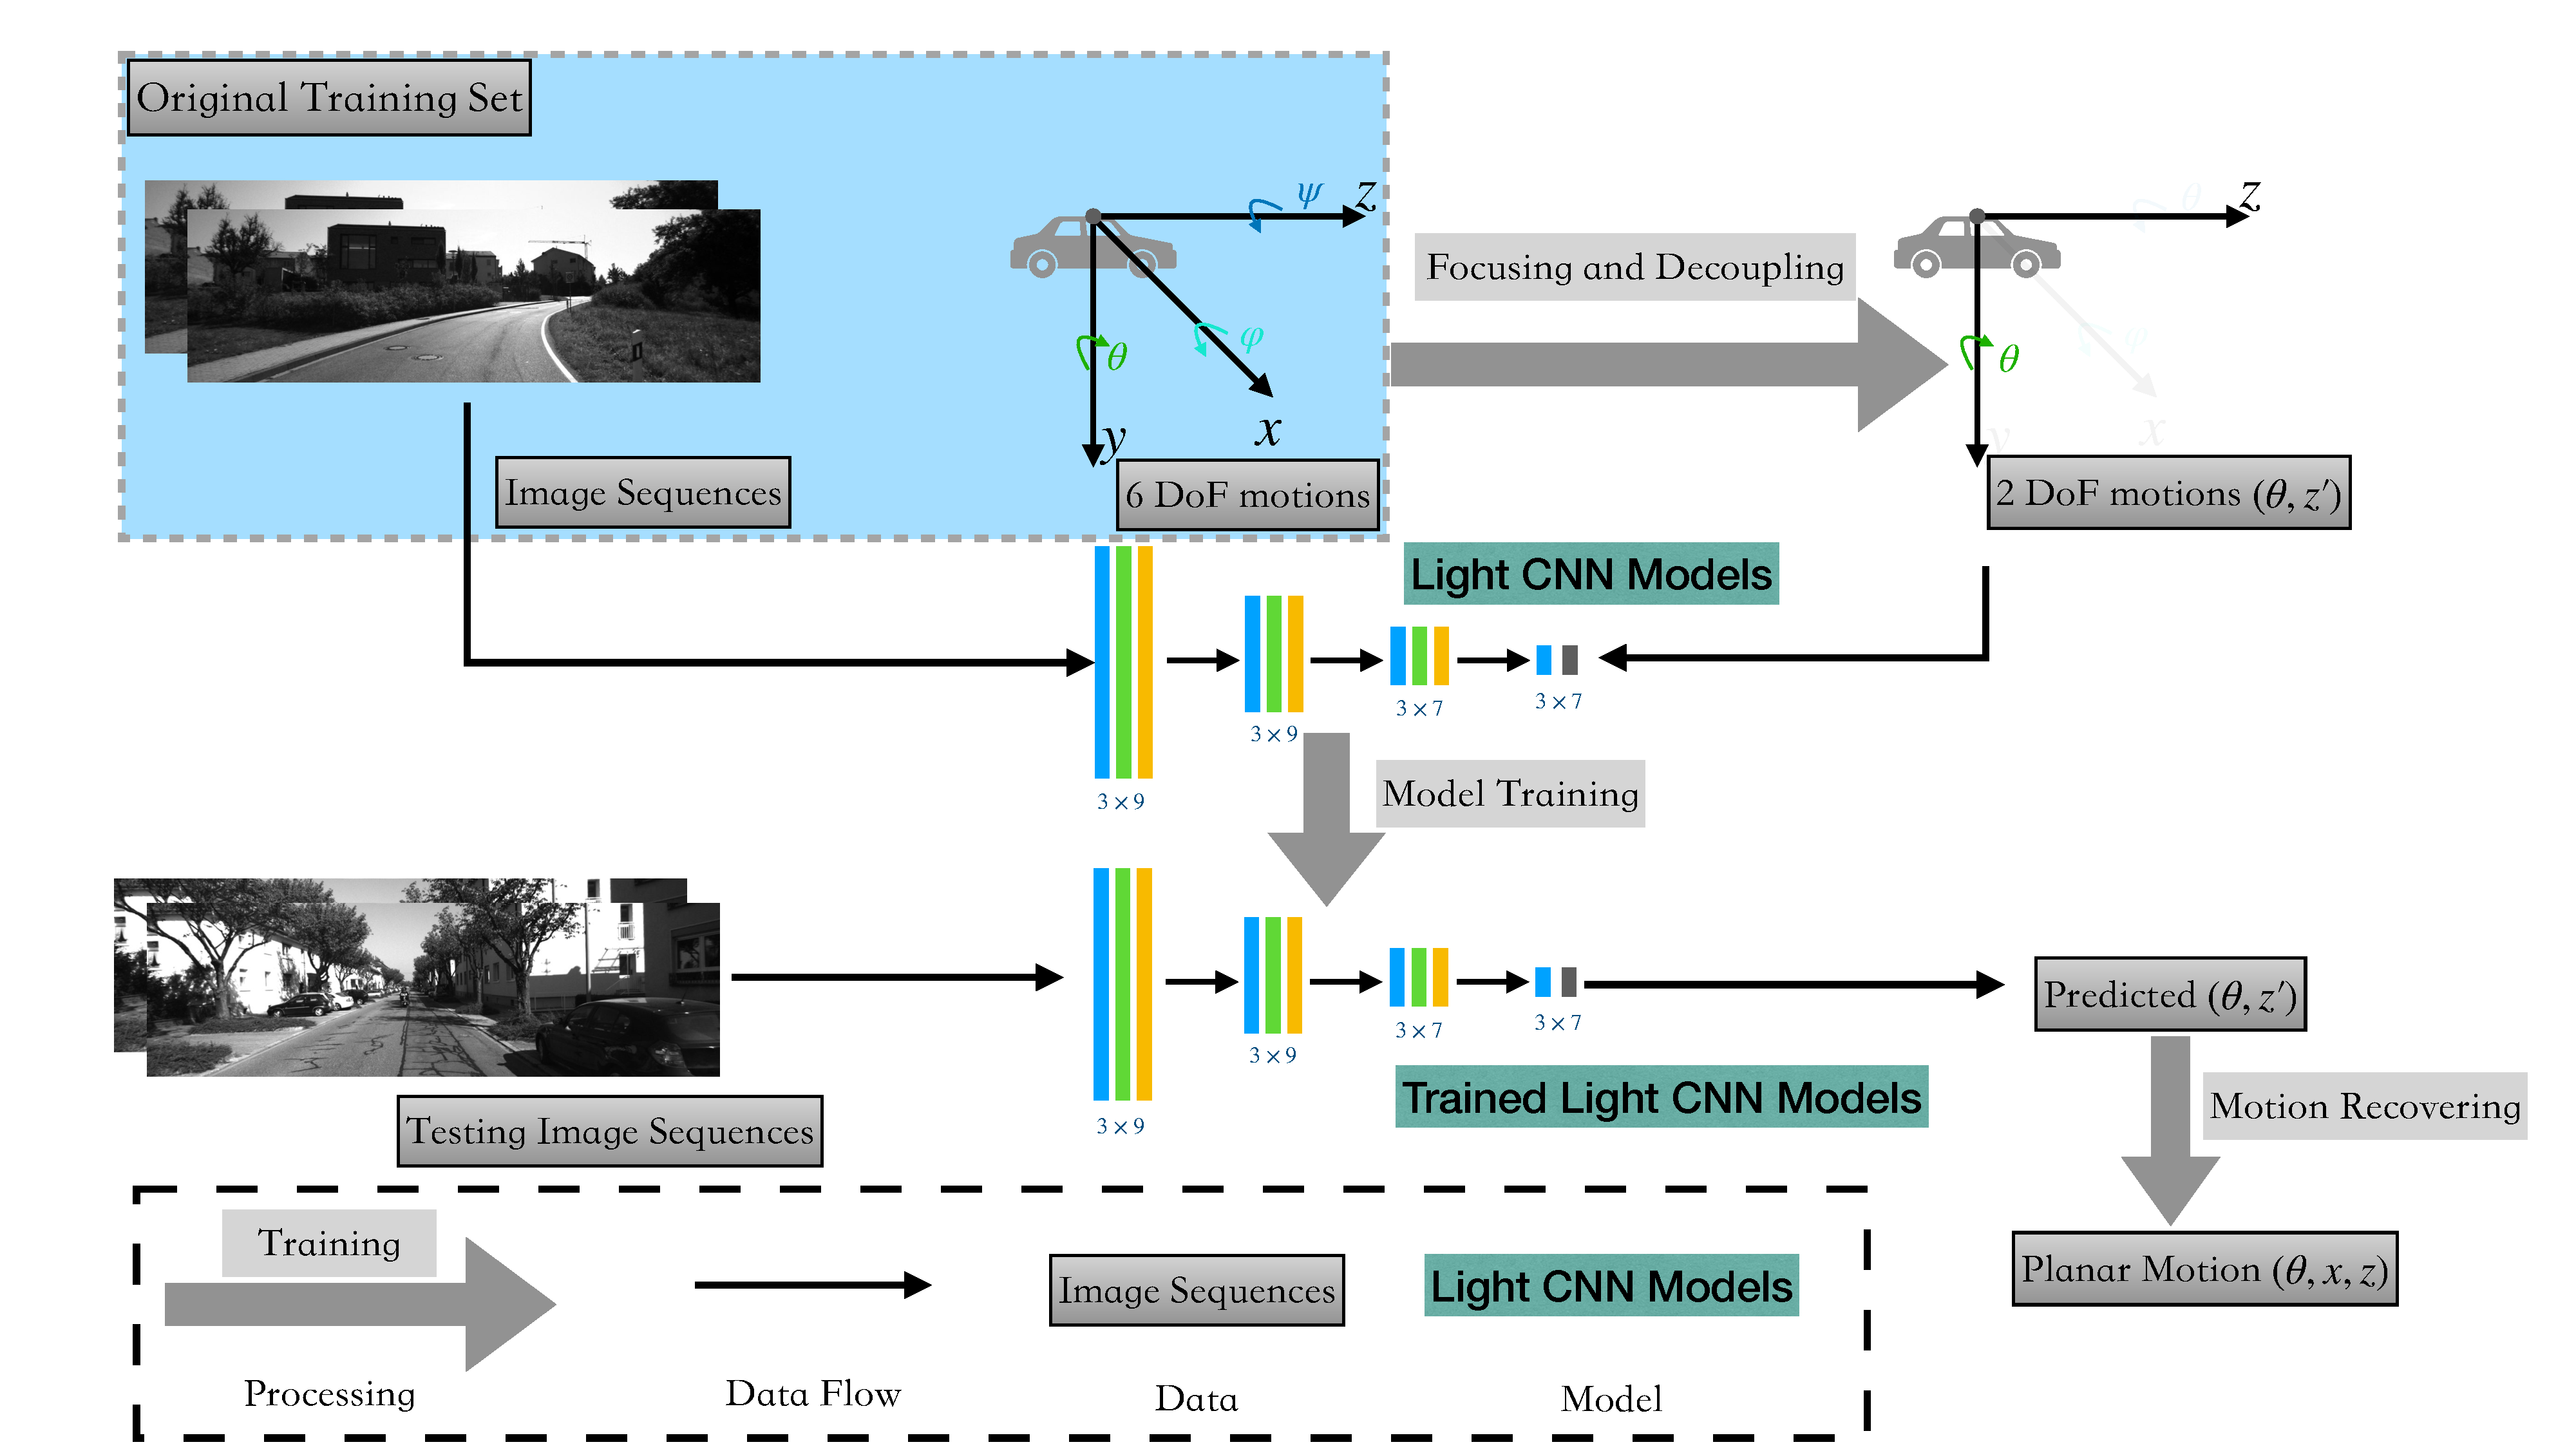
\includegraphics[width=0.9\textwidth]{datavo/system_structure.pdf}
    \caption{运动聚焦与解耦算法系统结构。}
    \label{fig:system_structure}
\end{figure*}
本节在\ref{sec:motion}首先介绍了运动聚焦和运动解耦的数据处理方法;然后在章节\ref{sec:model}中介绍了关于地面车辆视觉里程模型的网络结构和训练细节。

%\subsection{Data Processing}
\subsection{运动聚焦和运动解耦}
\label{sec:motion}
运动聚焦是通过将注意力集中在主要运动上来简化学习目标的一种思想,这在\ref{sec:motion_focus}中有详细描述,运动聚焦引起的姿势位移在节\ref{sec:info_loss}中进行了评估。运动解耦减少了运动聚焦引起的姿势位移,
这在\ref{sec:motion_decouple}中进行了描述,在\ref{sec:info_decouple}中进行了定量评价。运动聚焦和运动解耦引起的性能提升在\ref{sec:ego_improvement}节中进行评估。
\subsubsection{运动聚焦}
\label{sec:motion_focus}
\begin{figure}[ht]
    \centering
    \begin{subfigure}[b]{0.65\textwidth}
        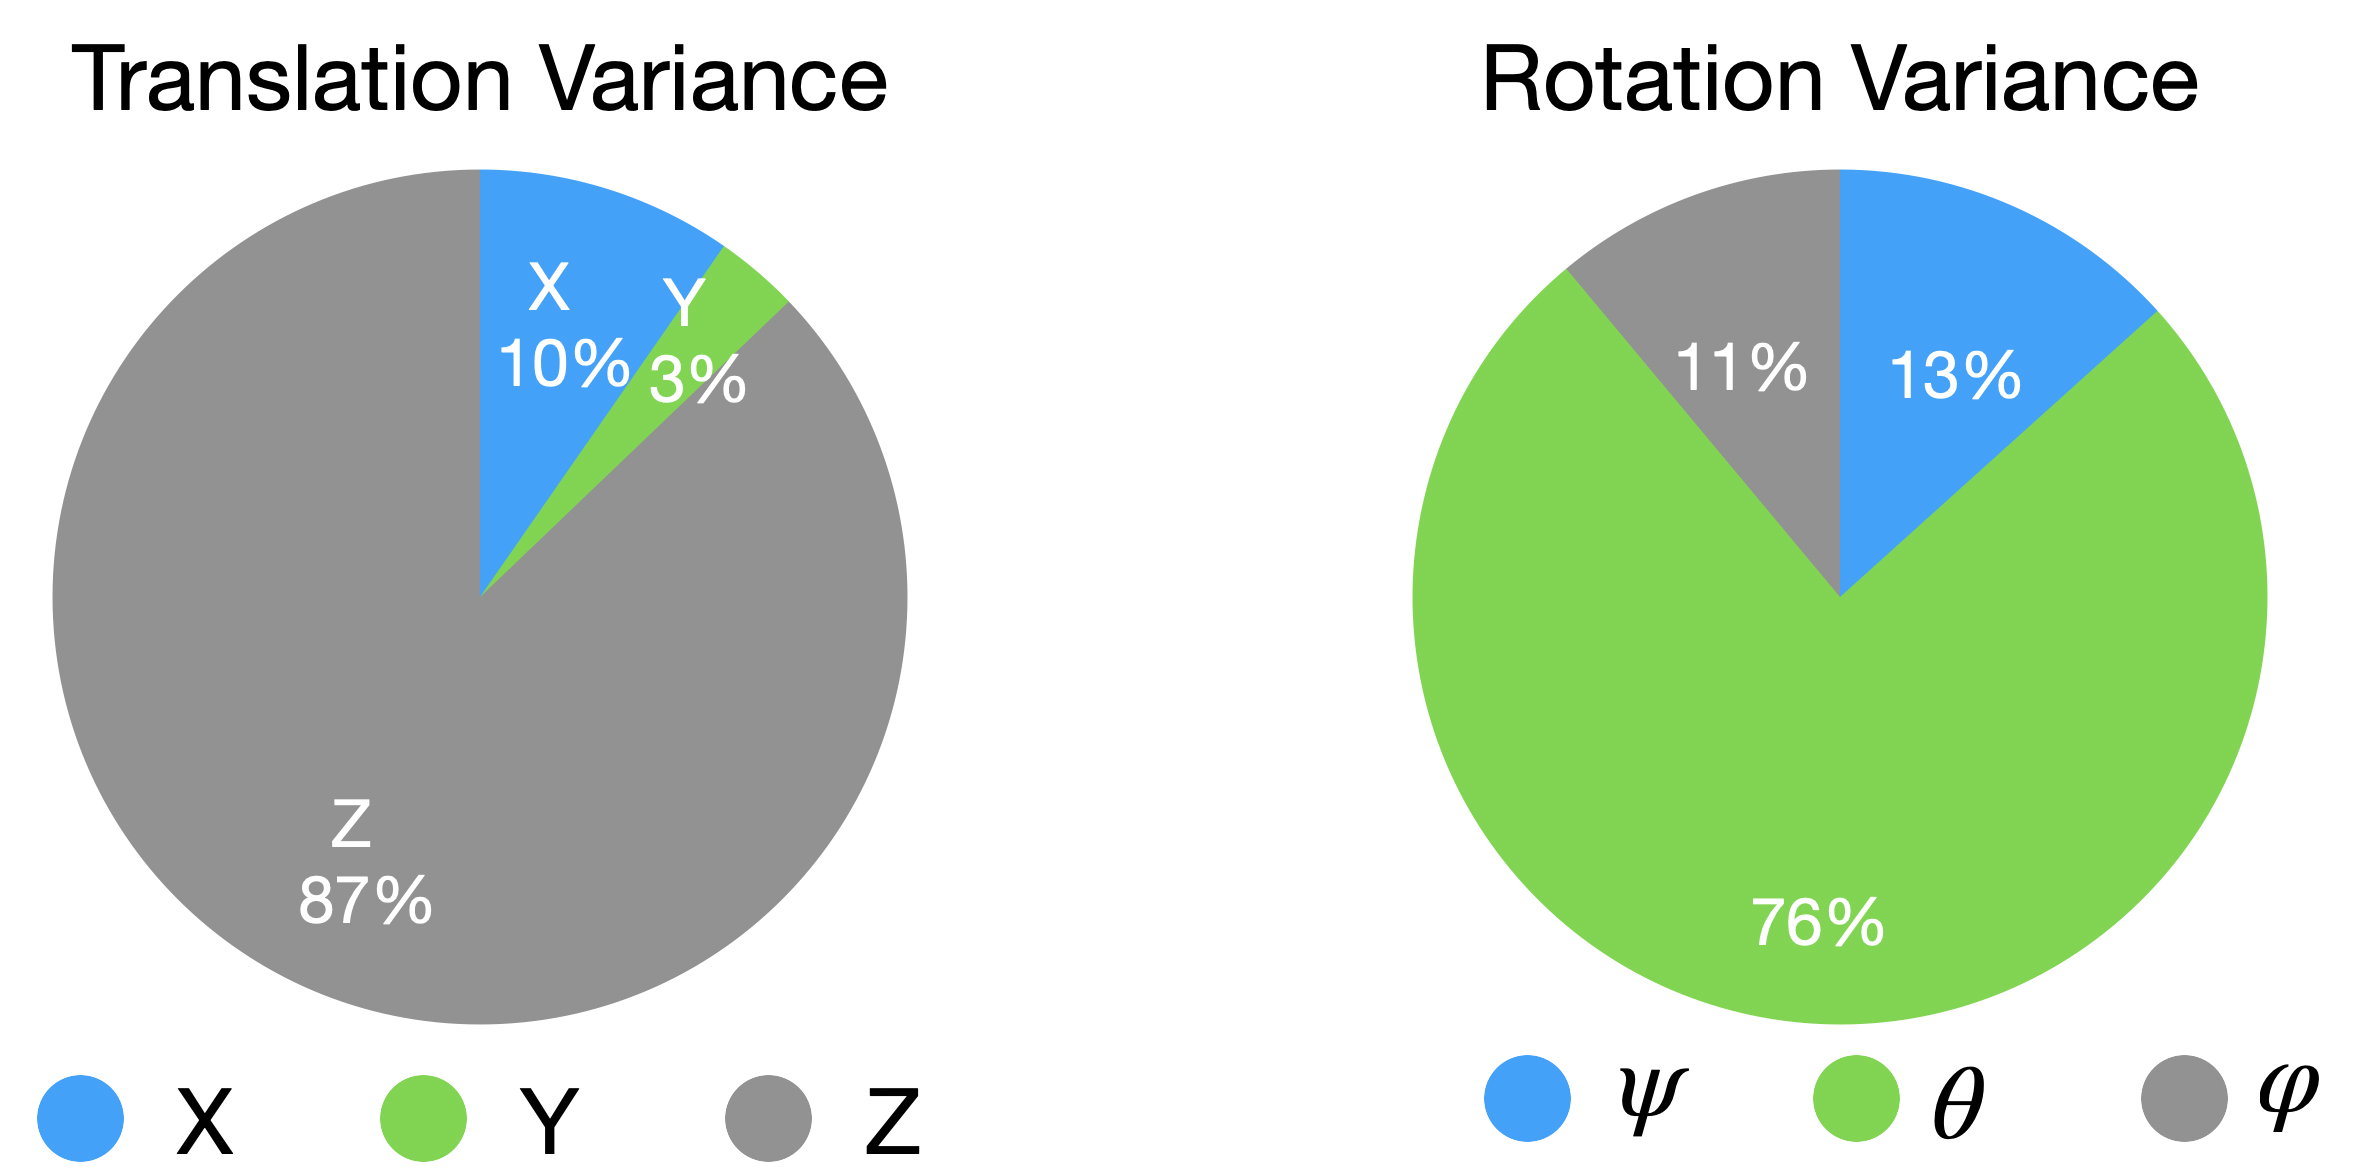
\includegraphics[width=\textwidth]{datavo/motion_dis.png}
        \caption{}
        \label{fig:motion_dis} 
        \vspace{4pt}
    \end{subfigure}
    \begin{subfigure}[b]{0.65\textwidth}
        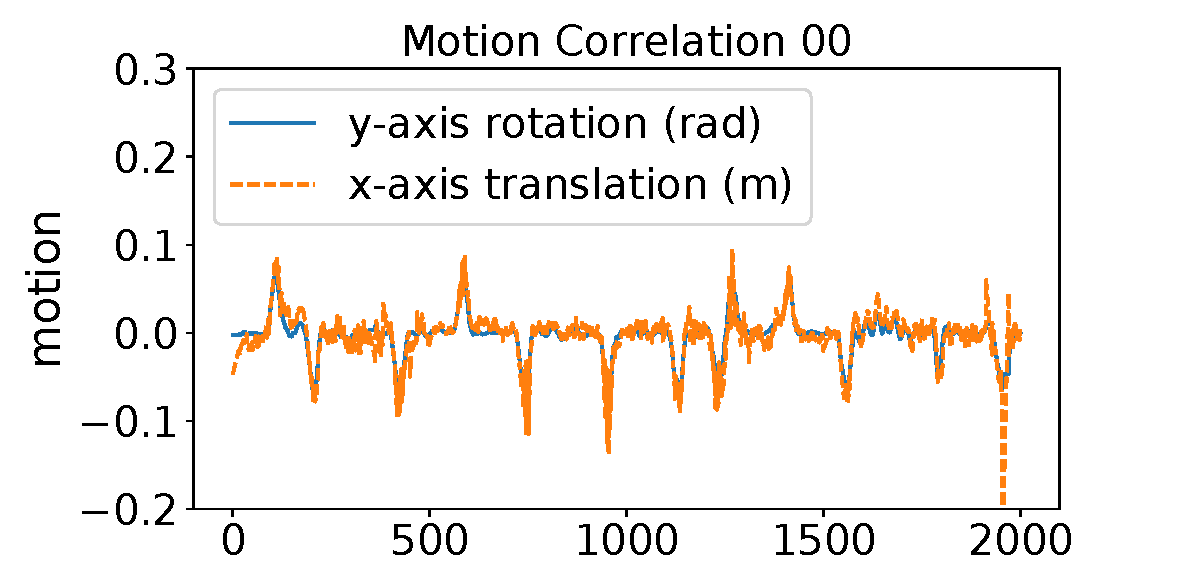
\includegraphics[width=\textwidth]{datavo/rotation_corr.pdf}
        \caption{}
        \label{fig:rotation_corr}
    \end{subfigure}
        \caption{运动模式分析。(a)沿着或围绕不同轴的运动比较;(b)X轴平移和Y轴旋转的相关性。}
\end{figure}

%The common method to deal with motion amplitude difference is data normalization or using different loss scale parameters \cite{wang2017deepvo}. 
%However, because the signal-noise ratio is small for the constraint motion axis of a ground vehicle,
%the normalization will introduce a lot of noise. 
运动聚焦就是忽略地面车辆的微不足道的运动,集中精力对大部分运动进行建模。我们在分解运动时采用常规的相机坐标系作为参考系(如图\ref{fig:car_simplify}所示),
该坐标系为右手系,定义如下:原点为相机的光学中心,z轴定义为前进光轴,x轴水平向右,y轴垂直向下。
围绕x轴、y轴和z轴的旋转运动分别用Euler角$\psi$、$\varphi$和$\theta$表示。沿不同轴的平移运动分别用$x$、$y$和$z$表示。

\begin{figure}[h]
    \centering
    \begin{subfigure}[b]{0.65\textwidth}
        \centering
        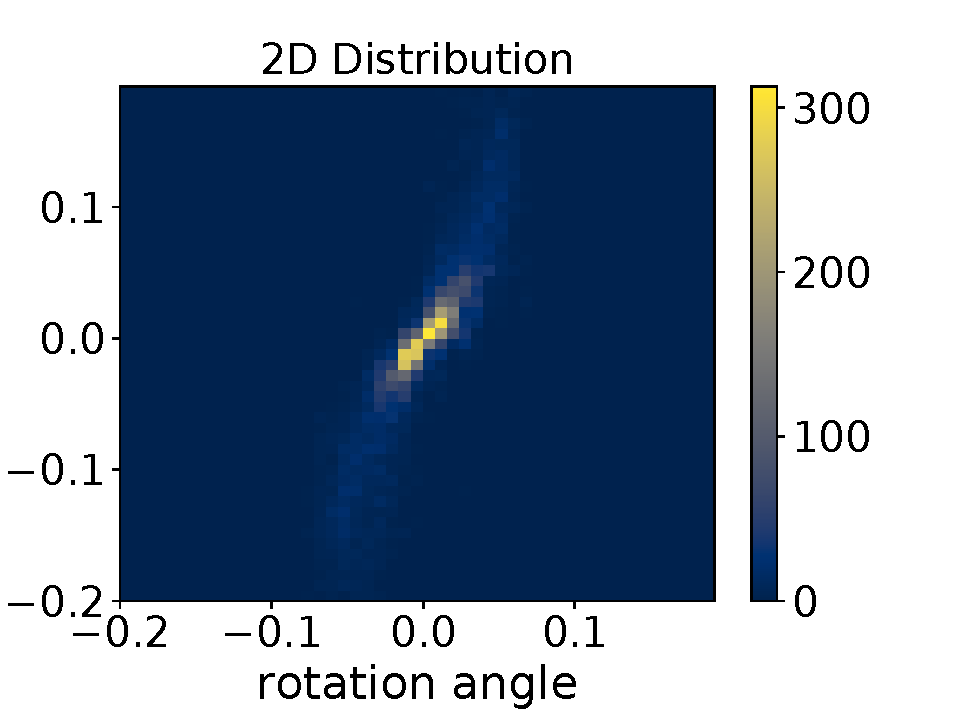
\includegraphics[width=\textwidth]{datavo/r_t_2d_hist.pdf}
        \caption{}
        \label{fig:rt_2d} 
        \vspace{4pt}
    \end{subfigure}
    \begin{subfigure}[b]{0.65\textwidth}
        \centering
        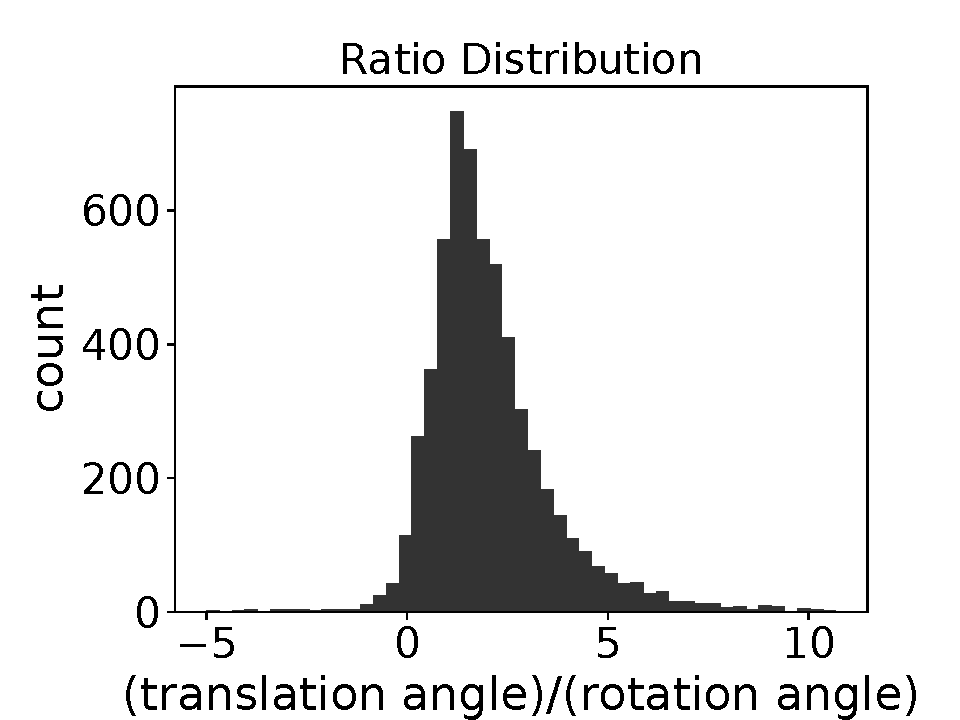
\includegraphics[width=\textwidth]{datavo/r_t_1d_hist.pdf}
        \caption{}
        \label{fig:rt_1d}
    \end{subfigure}
    \caption{旋转角和平移角的关系。(a)平移角和旋转角的二维直方图;(b)平移角和旋转角的一维直方图。}
    \label{fig:rotation_corr_analysis}
\end{figure}
我们在一个典型的地面车辆运动估计数据集——KITTI视觉里程数据集\cite{geiger2012kitti}上对地面车辆的运动模式进行了定量评估。
我们计算了KITTI序列00中关于不同轴的平移运动和旋转运动的方差,如图\ref{fig:motion_dis}所示,更多的方差可视化与图\ref{fig:motion_dis}类似,详见附录。
图\ref{fig:motion_dis}显示了地面车辆的大部分运动是z轴方向的平移运动和y轴方向的旋转运动。
所以我们建议简化运动估计目标,只关注大多数运动,我们称这个建议为运动聚焦。由运动聚焦引起的姿势位移在第\ref{sec:info_loss}节中进行了评估。

\subsubsection{运动解耦}
\label{sec:motion_decouple}

然而,如图\ref{fig:motion_dis}所示,沿x轴仍有不可忽略的平移运动,具体分析见表\ref{tab:info_loss_1}。
由此可知,如果直接全部忽略X轴的运动,会造成较大的漂移姿势(10\%)。然而,考虑到动力学约束,地面车辆不能沿X轴移动太多,为什么
存在高达10%的X轴平移呢?当深入研究地面车辆的运动模式时,我们发现X轴运动是由运动表示方法产生的。
\begin{equation}
    \begin{pmatrix} \mathbf{R} & \mathbf{t}\\ 0 & 1  \end{pmatrix} = \begin{pmatrix} \mathbf{I}& \mathbf{t}\\ 0 & 1  \end{pmatrix}\begin{pmatrix} \mathbf{R}& \mathbf{0}\\ 0 & 1  \end{pmatrix}
    \label{eq:ftlr}
\end{equation}
这里$\mathbf{I}$是一个3x3的单位矩阵。
在这种表示方式中,平移运动$mathbf{t}$先于旋转运动$mathbf{R}$。因此,当车辆有旋转运动时,参考坐标系统已经发生了变化,前向运动$z'$
被映射成较小的前向运动$z$与侧向运动(x轴平移{$x$}),如图\ref{fig:vehicel_rotation_model}所示。它引起的平移角$\alpha$,定义为: 
\begin{equation}
    \alpha = \arctan\left(\frac{x}{z}\right)
\end{equation}
这里$x$和$z$分别表示x-轴与z-轴的平移。
当我们将x轴平移和y轴旋转可视化后,就可以得到验证,如图\ref{fig:rotation_corr}所示,因为这两个运动是高度相关的。图\ref{fig:rotation_corr}只能可视化一个子序列的局部相关性。我们利用图\ref{fig:rotation_corr_analysis}中的两个直方图来可视化KITTI数据集序列00-10中,所有Y轴旋转角$\theta$和平移角$\alpha$的全局关系。
我们利用图中的两个直方图(\ref{fig:rotation_corr_analysis})来可视化所有KITTI序列00-10中所有Y轴旋转角$theta$和平移角$alpha$的全局关系。图\ref{fig:rt_1d}中的1d直方图显示了$\alpha/\theta$的分布,图\ref{fig:rt_2d}中的2d直方图可视化了$\alpha$和$\theta$的联合分布。这两个分布都表明y轴的旋转角$\theta$和平移角$\alpha$是相关的。
那么如何重新制定运动表示法来减少运动的相关性呢?一个简单的方法是将平移重写为:
\begin{equation}
    \begin{pmatrix} \mathbf{R} & \mathbf{t}\\ 0 & 1  \end{pmatrix} = \begin{pmatrix} \mathbf{R'}& \mathbf{0}\\ 0 & 1  \end{pmatrix}\begin{pmatrix} \mathbf{I}& \mathbf{t'}\\ 0 & 1  \end{pmatrix}
    \label{eq:frlt}
    \end{equation}
在这个公式中,车辆的旋转是先于平移的,所以平移运动是相对于旋转运动后的参考系而言的,不会被重新映射。可以得出的关系是:
$\mathbf{R'} = \mathbf{R}$, $\mathbf{t'} = \mathbf{R}^{-1}\mathbf{t}$.
\begin{figure}[ht]
    \centering
    \begin{subfigure}[b]{0.65\textwidth}
        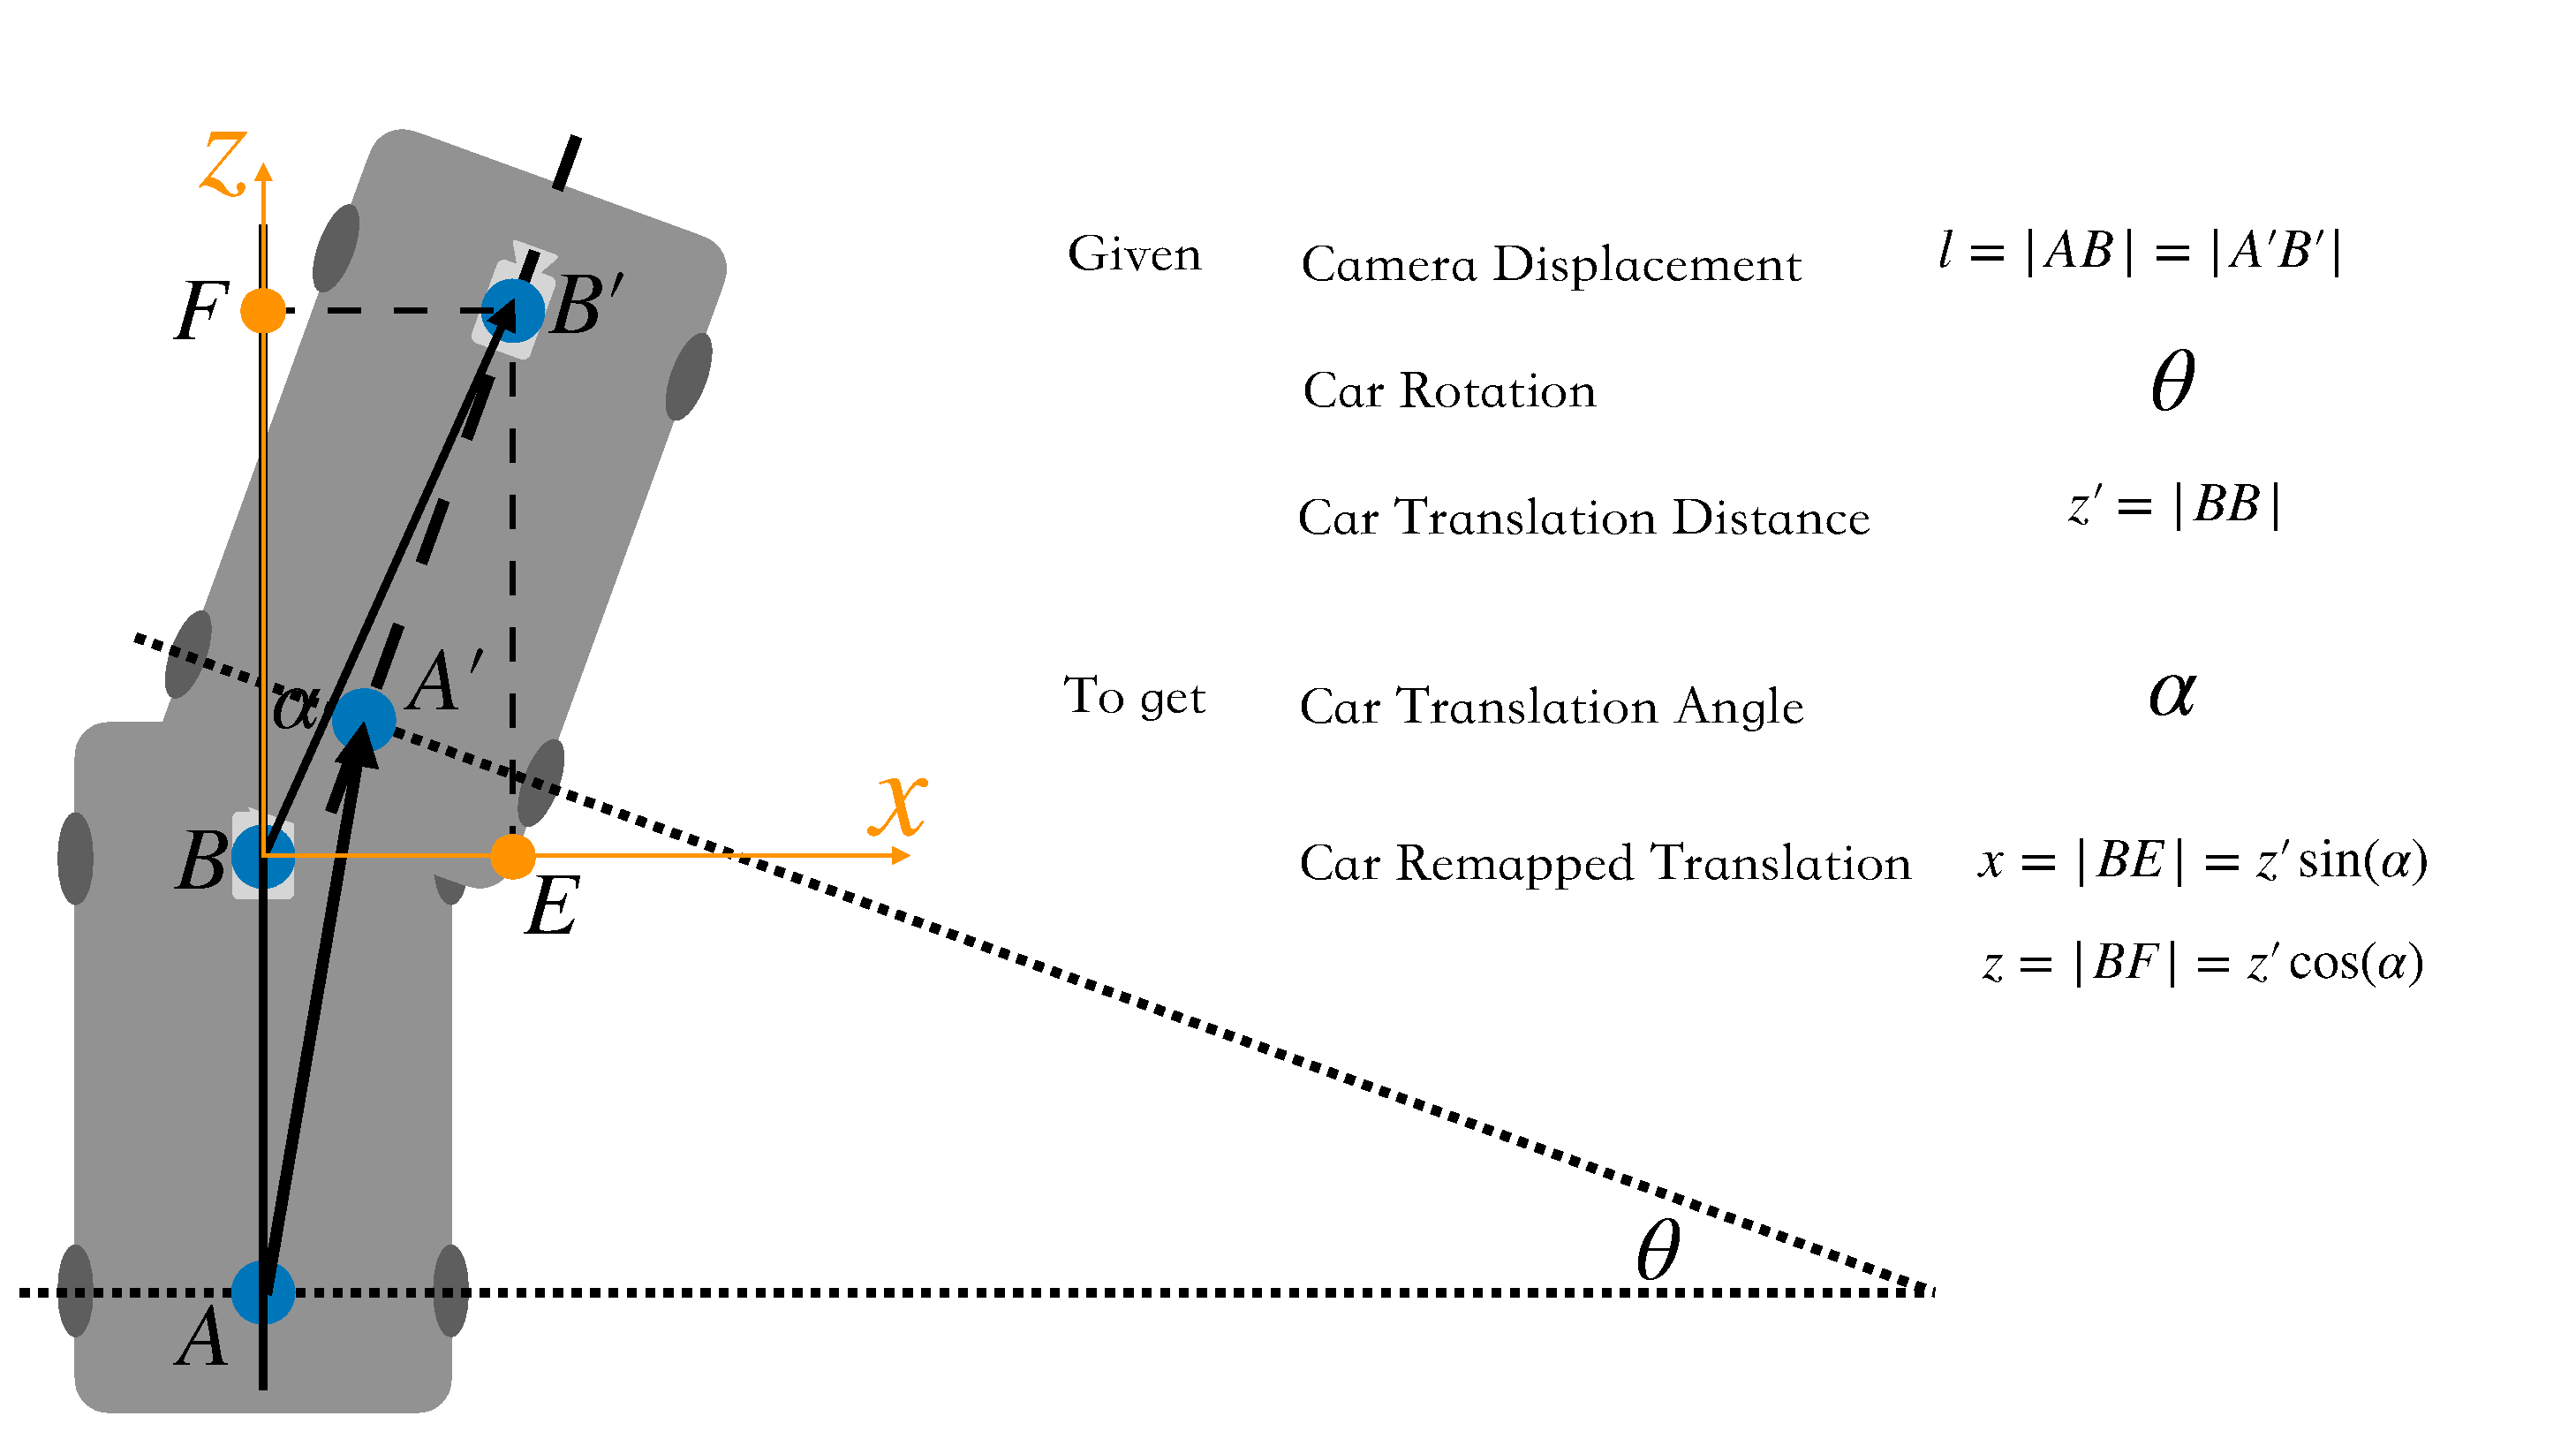
\includegraphics[width=\textwidth]{datavo/vehicle_rotation_1-crop.pdf}
        \caption{}
        \label{fig:vehicel_rotation_model} 
        \vspace{4pt}
    \end{subfigure}
    \begin{subfigure}[b]{0.6\textwidth}
        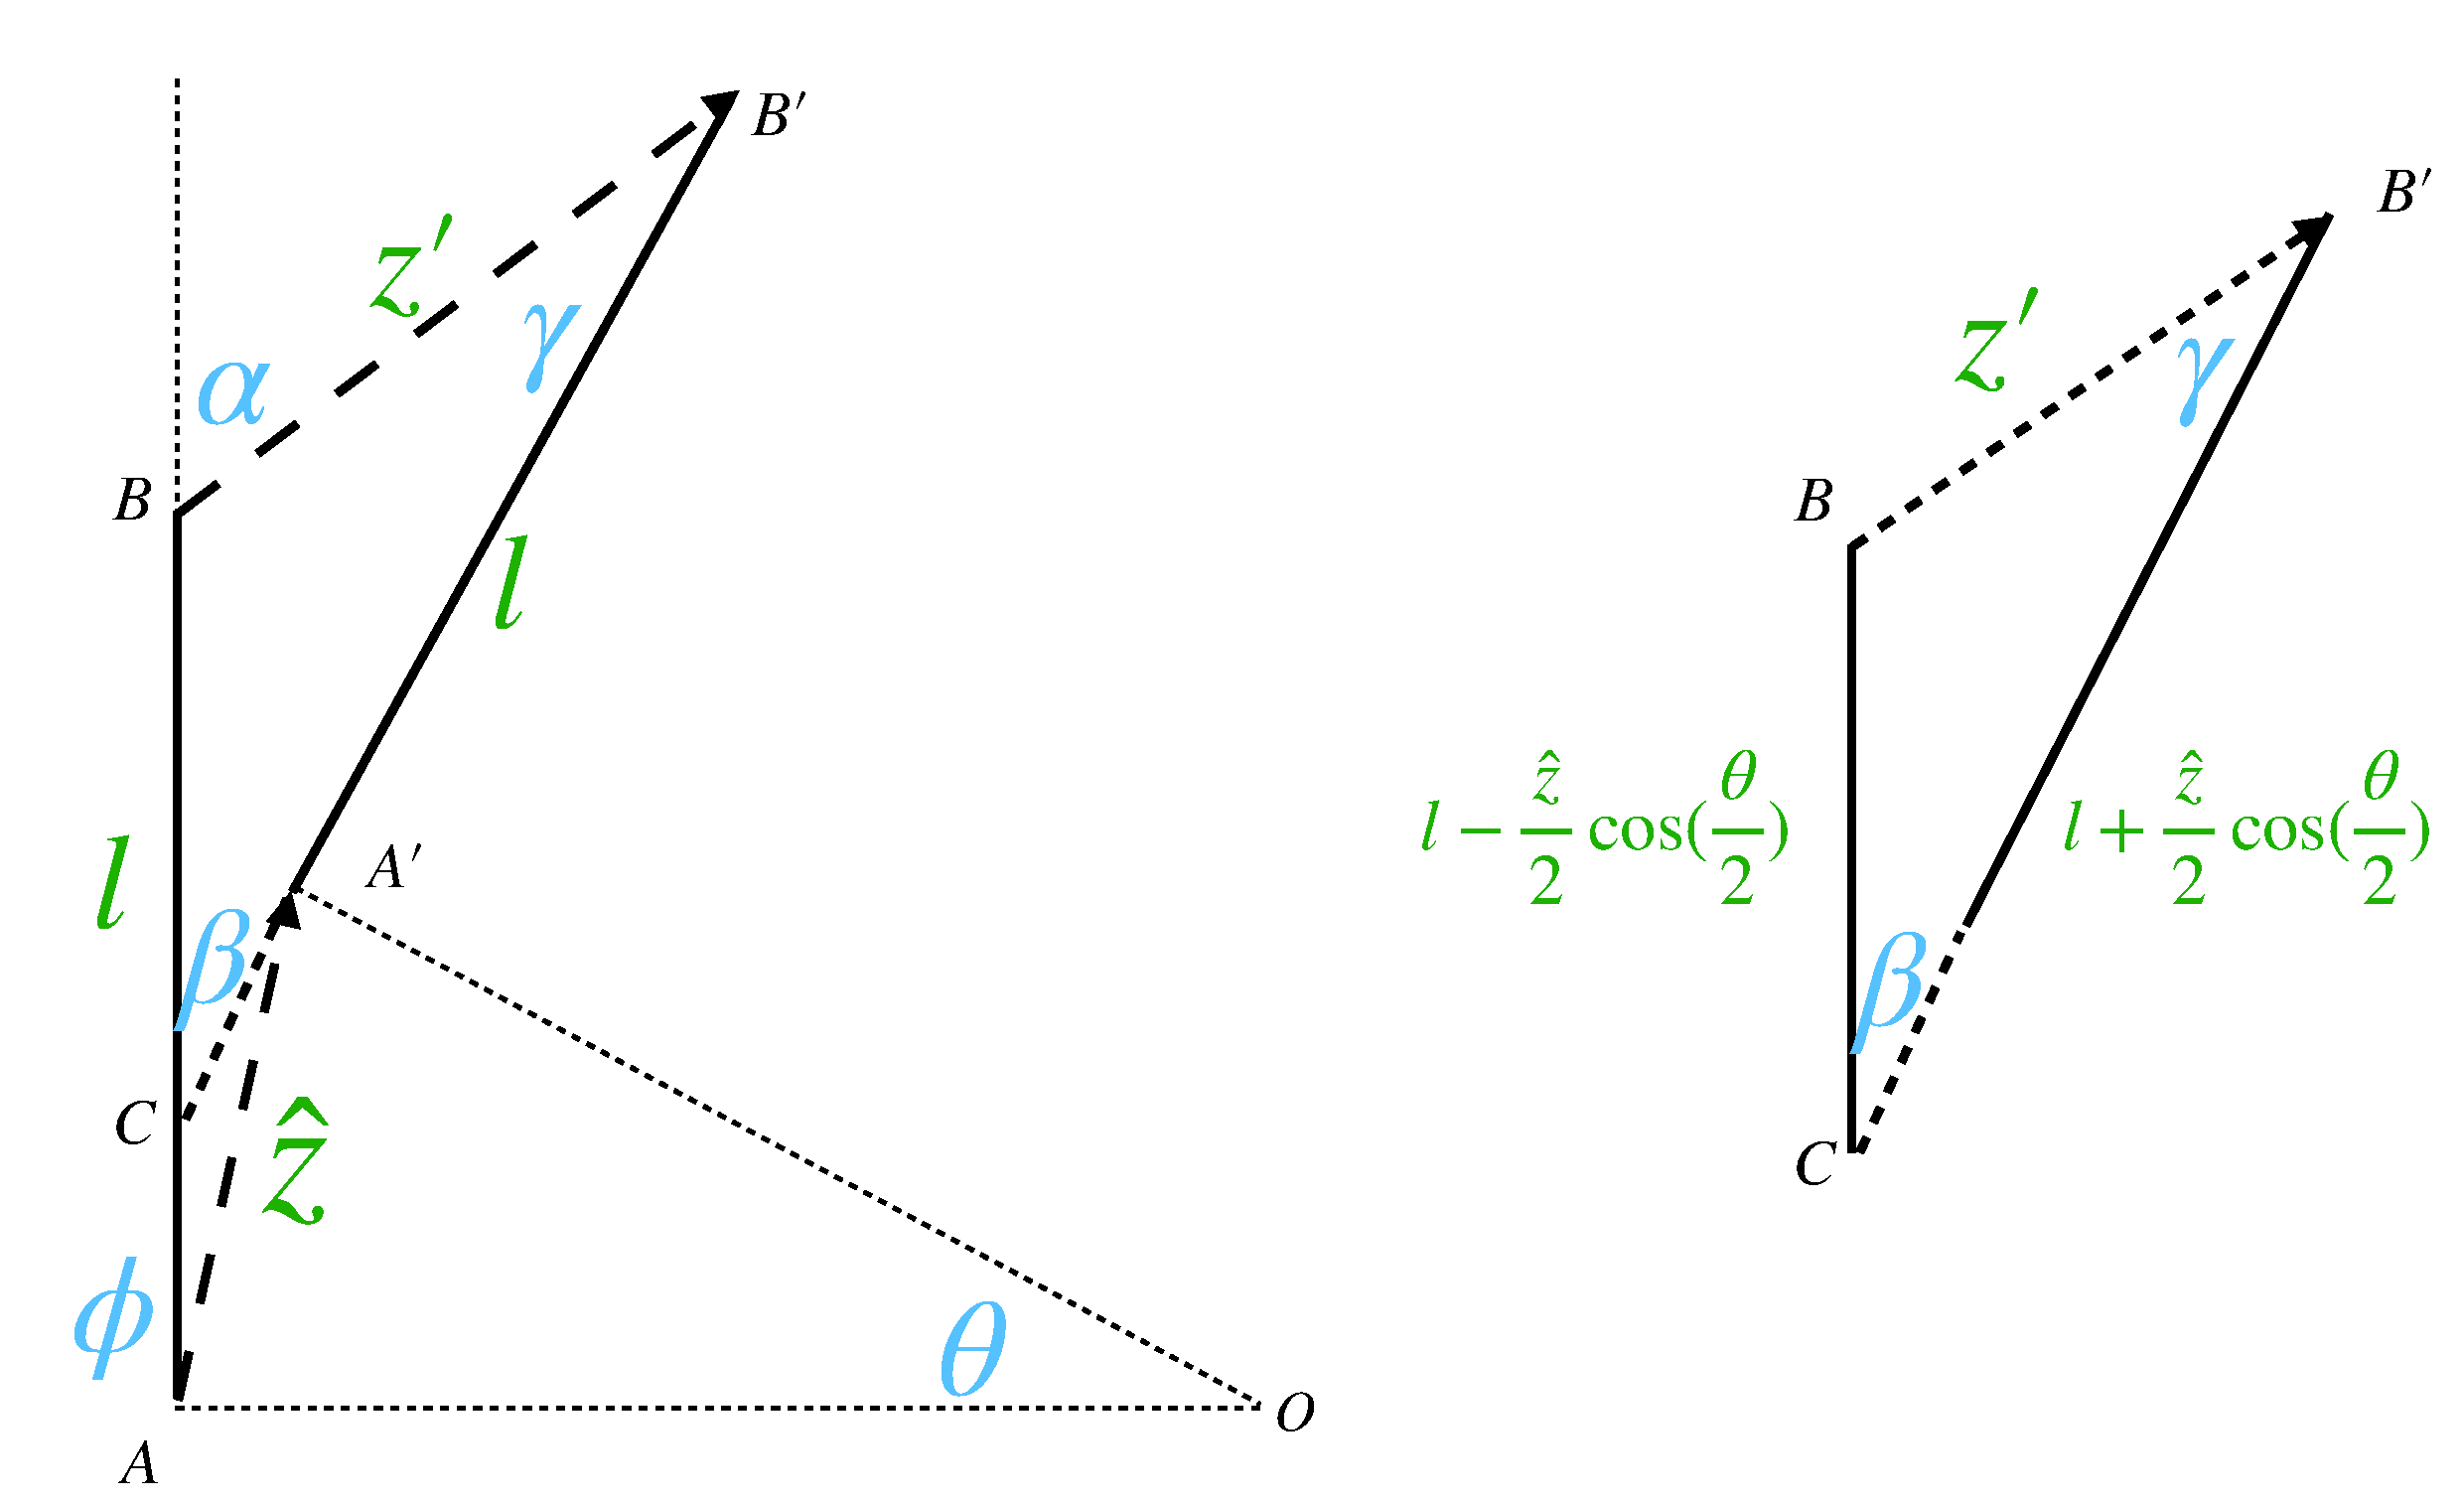
\includegraphics[width=\textwidth]{datavo/vehicle_rotation_2-crop.pdf}
        \caption{}
        \label{fig:vehicel_rotation_model_s} 
    \end{subfigure}
    \caption{地面车辆旋转模型。(a) 旋转模型;(b) 简化的旋转模型。}
    \label{fig:rotation_model}
\end{figure}
然而,如图\ref{fig:vehicleel_rotation_model}所示,绕y轴的旋转角度$\theta$不等于由旋转产生的平移角$\alpha$。
我们需要找出$\alpha$和$\theta$之间的关系$\alpha=f(\theta)$。
然后,我们就只需保持y轴的旋转$\theta$和汽车的前移$z$,使用平移角$\alpha$,用公式\eqref{eq:car_angle}来恢复车辆的运动。
\begin{equation}
    (x,z) = z'(sin(f(\theta)),cos(f(\theta)))
    \label{eq:car_angle}
\end{equation}
在图\ref{fig:vehicleicel_rotation_model}中,A点是车辆后轴的中心,标记B是安装摄像头的位置,$l$表示A和B之间的距离。通过视觉里程测量法估算出的
车辆平移距离等于$B$和$B'$之间的距离,用{$z'$}表示。我们将图\ref{fig:vehicleel_rotation_model}简化为图\ref{fig:vehicleel_rotation_model_s}。
根据阿克曼转向定律\cite{siegwart2011introduction},$OA \bot AB$且$OA' \bot A'B'$,所以$\phi = 0.5 \beta = 0.5 \theta$。
在三角形$CBB'$中,根据正弦定律可知:
{
\begin{equation}
   \frac{\sin(\gamma)}{\sin(\beta)}  = \frac{l-\frac{\hat{z}}{2} / \cos(\frac{\theta}{2})}{z'} 
\end{equation}}
因为$\theta$趋近于0,所以$\cos(\frac{\theta}{2}) \approx 1$,且$ \frac{\gamma}{\beta} \approx  \frac{\sin(\gamma)}{\sin(\beta)} $,因此
{
\begin{equation}
    \frac{\gamma}{\beta}  \approx \frac{l-\frac{\hat{z}}{2}}{z'} 
\end{equation}}
又根据三角形$CBB'$中的余弦定律,{$d = |AC| \approx 0.5|AA'| =0.5\hat{z}$}
{
\begin{equation}
    \begin{split}
        z'^2 &= (l+d)^2 + (l-d)^2- 2(l+d)(l-d)\cos(\beta) \\
        &= 2l^2+2d^2 - 2(l^2-d^2)\cos(\beta)\approx 4d^2
    \end{split}
\end{equation}
}
因此$z'\approx \hat{z}$,可知平移角度$\alpha$和旋转角度$\theta$
{
\begin{equation}
    \alpha = \beta + \gamma \approx (\frac{l}{z'}+0.5)\beta =(\frac{l}{z'}+0.5)\theta
    \label{eq:r_t_ratio}
\end{equation}}
我们用位移角度$a$构建旋转矩阵$\mathbf{R}_\alpha$,
\begin{equation}
    \mathbf{R}_\alpha = \begin{pmatrix}
        \cos(\alpha)& 0 & \sin(\alpha)\\ 
        0 & 1 & 0\\ 
        -\sin(\alpha)& 0 & \cos(\alpha)\\ 
    \end{pmatrix} 
    \label{eq:r_alpha}
\end{equation}
然后得到$\mathbf{t}'$变形为
\begin{equation}
    \mathbf{t}' = \mathbf{R}_\alpha^{-1}\mathbf{t}
    \label{eq:decouple_z}
\end{equation}
所需的车辆前行运动{$z'$}是$\mathbf{t}'$的第三个元素。到目前为止,地面车辆的规划者运动可以由两个变量来表示:旋转角$\theta$和重映射前向运动$z'$。
我们专注于学习两维运动,以简化学习目标。模型和学习细节将在下一节介绍,运动聚焦和解耦引起的性能提升将在\ref{sec:ego_improvement}中进行评估。

\subsection{模型与训练}
\label{sec:model}
\begin{figure*}[t]
    \centering
    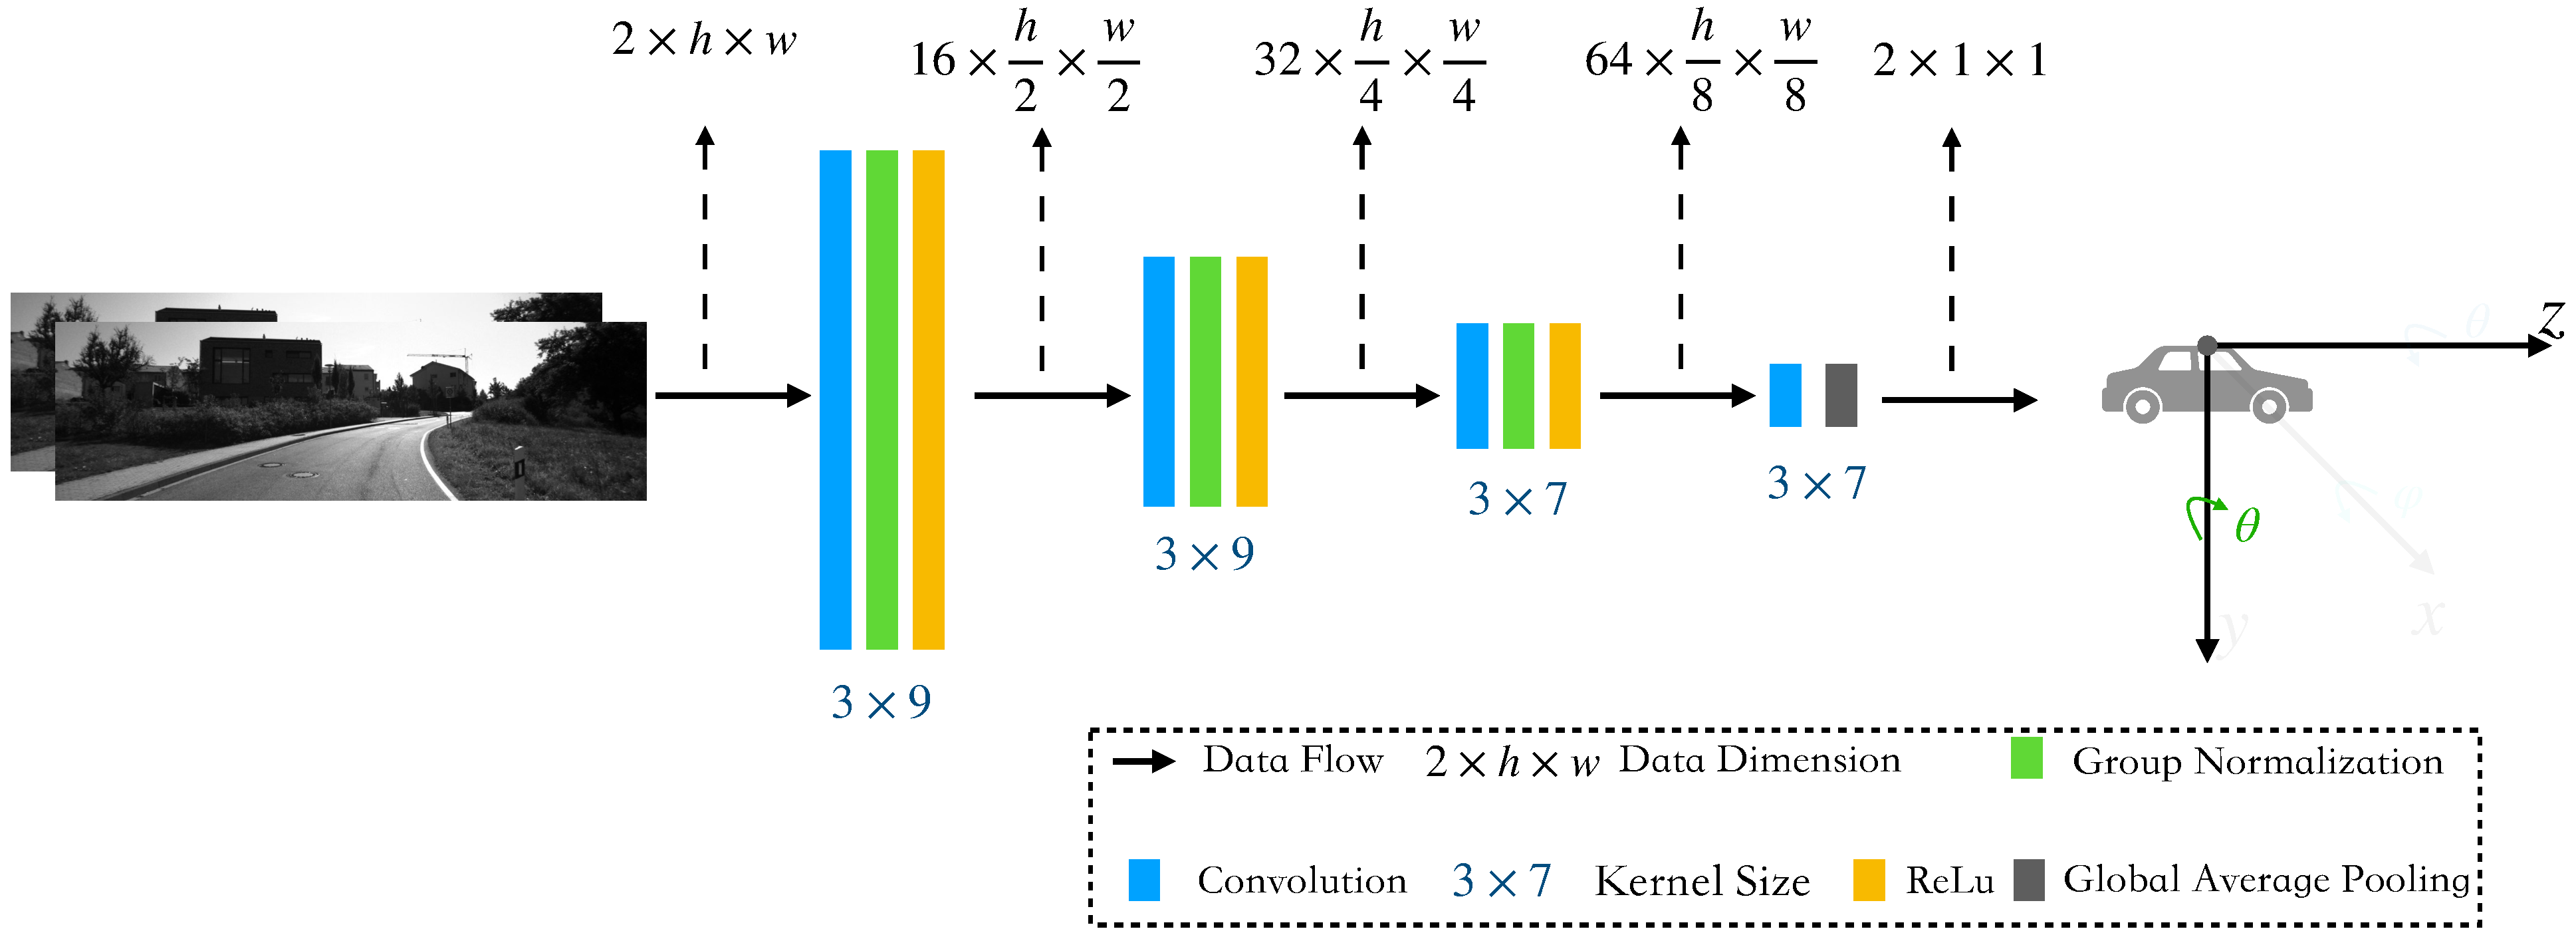
\includegraphics[width=\textwidth]{datavo/network_structure_2-crop.pdf}
    \caption{自我运动估计的轻型卷积神经网络}
    \label{fig:nerwork_structure}
\end{figure*}
我们构建一个轻型网络结构来学习地面车辆的主要运动。如图\ref{fig:nerwork_structure}所示。模型主要由卷积层组成,除了最后一层外,每个卷积层后面都有一个
组归一化层\cite{wu2018group}和ReLU层。与Zhou等人相同的是\cite{zhou2017unsupervised},我们使用全局平均池化层\cite{lin2013network}而不是全连接层
作为最后一层,以减少过拟合。我们观察到,地面车辆拍摄的图像的光流主要是水平的,特别是当车辆转弯时,如图\ref{fig:optical_flow}所示,所以我们利用卷积层与非
正方形核来实现更大的水平感受野。此外,我们还采用了扩张卷积层\cite{yu2015multi},以较少的参数获得更大的感知场。
\begin{figure}[ht]
    \centering
    \begin{subfigure}[b]{0.45\textwidth}
        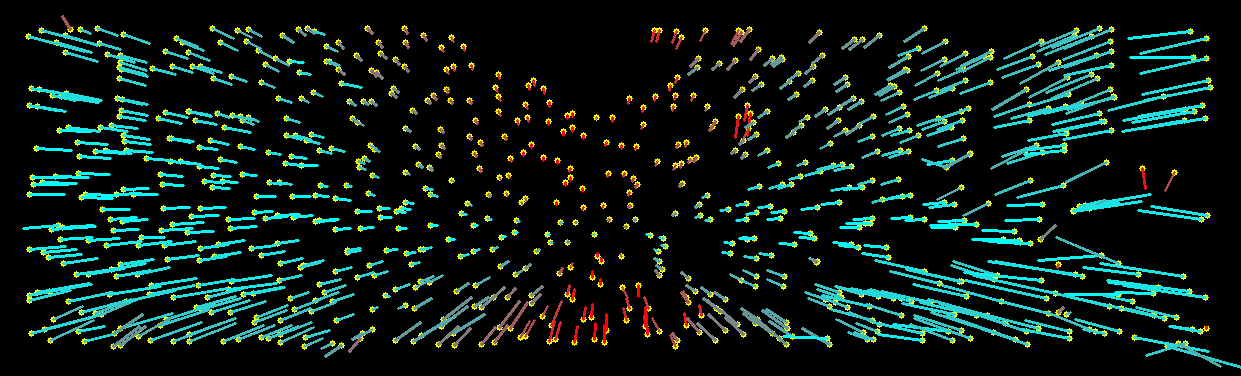
\includegraphics[width=\textwidth]{datavo/flow_61.png}
        \caption{}
        \label{fig:optical_flow_f} 
        \vspace{4pt}
    \end{subfigure}
    \begin{subfigure}[b]{0.45\textwidth}
        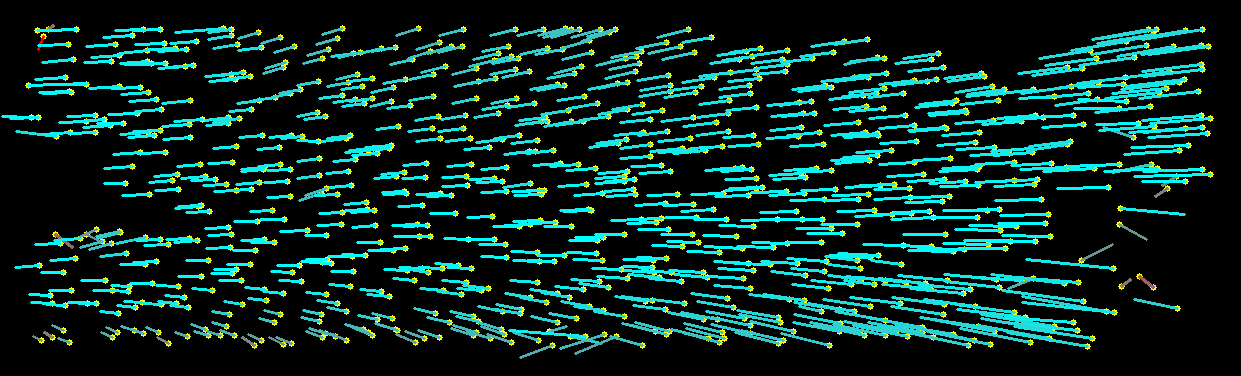
\includegraphics[width=\textwidth]{datavo/flow_196.png}
        \caption{}
        \label{fig:optical_flow_l} 
        \vspace{4pt}
    \end{subfigure}
    \begin{subfigure}[b]{0.45\textwidth}
        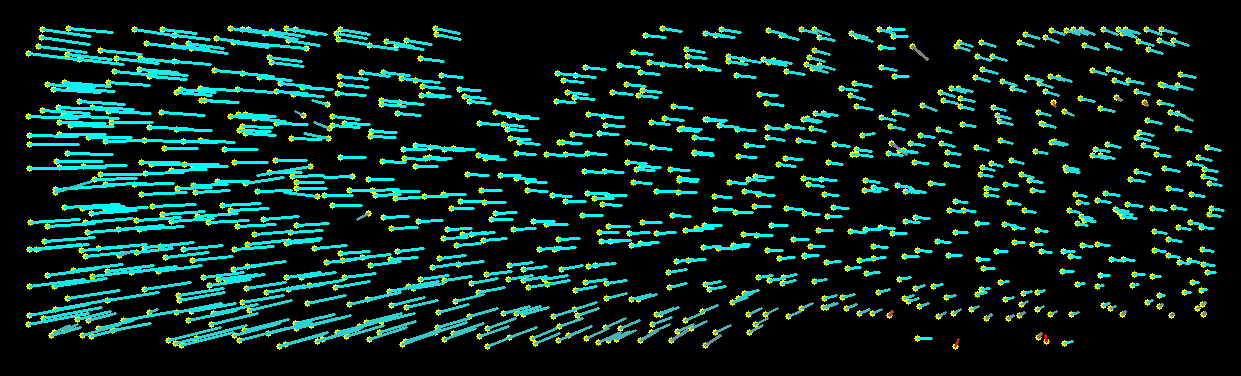
\includegraphics[width=\textwidth]{datavo/flow_96.png}
        \caption{}
        \label{fig:optical_flow_r} 
    \end{subfigure}
    \caption{地面车辆的光流。(a) 前进时的光流;(b) 左转时的光流;(c) 右转时的光流。}    
    \label{fig:optical_flow}
\end{figure}

模型的输入是堆叠的灰色图像对,我们不仅使用序列图像来构造图像对{(帧间隔为0)},而且在{[-4,4]}中为每个样本随机选择一个{帧间隔},作为一个数据{增量}过程。 

输出是由y轴旋转$\theta $和重映射前向平移$z'$所代表的相应主要相机运动。  {$z'$是根据\eqref{eq:decouple_z}}得到的。
L2损失被用作监督函数:
\begin{equation}
    L_2 = \|\theta_g -\theta_p\|_2 +\|z'_g -z'_p \|_2
\end{equation}
下标为$p$的变量$\theta_p$和{$z'_p$}代表预测的{结果},下标为$g$的变量$\theta_g$和{$z'_g$}代表{the}地面真值。
我们使用ADAM \cite{kingma2014adam}来优化模型参数,学习率设置为0.001,50个epoch后线性衰减。%我们将权重衰减参数设置为0.001,以增加正则化。

模型训练完成后,输入一个新图像序列后,从模型输出中可以得到旋转角$\theta$和前向运动{$z'$}。
我们首先计算平移角$\alpha$,并假设关于其他轴的旋转为零,并构造旋转矩阵$\mathbf{R}_\theta$和$\mathbf{R}_\alpha$,则车辆转换向量{$\mathbf{t}_\alpha=\mathbf{R}_\alpha(0,0,z')^T$},该方程等同于\eqref{eq:car_angle},称为运动恢复。
路面车辆整体运动矩阵可以表示为: 
\begin{equation}
    \mathbf{T}_i =\begin{pmatrix} \mathbf{R}_\theta & \mathbf{t}_\alpha\\ 0 & 1  \end{pmatrix} 
    \label{eq:rt_final}
\end{equation}
然后,通过累积可以得到车辆位姿为: 
\begin{equation}
    \mathbf{P}_i = \mathbf{P}_{i-1}\mathbf{T}_i
    \label{eq:pose}
\end{equation}
\section{实验}
\label{sec:experiments}
我们在KITTI数据集\cite{geiger2012kitti}上进行了四个实验来评估所提出的方法的性能。首先,我们对KITTI数据集和实验平台进行介绍说明。
其次,我们详细介绍了四个实验:姿势位移评估、运动解耦性能、自我运动估计改进以及与其他方法的比较。最后,我们对实验结果进行讨论和分析。

\subsection{数据集和实验平台}

KITTI基准提供了22个测试序列,其中前11个序列为地面真实姿态评估。每个测试序列中都提供了{RGB图像、灰色图像和激光雷达点云}。


训练和测试我们的模型时,我们只利用单眼灰色图像与地面真实姿势{(KITTI数据集序列00-10)}。

{我们把训练数据集分成了四个不同的训练-评估模型,用于定量评估所提出的运动聚焦和解耦对自我运动估计的改进,详细内容见章节\ref{sec:ego_improvement};为了与其他相对方法进行比较,在章节\ref{sec:compare}中,我们使用KITTI 00-08进行训练,09-10进行评估,这与其他基于学习的方法是一样的,以便进行公平比较。} 

{我们使用RPE(相对姿势误差的简称)的平均值包括
相对旋转误差和相对位移误差 \cite{geiger2012kitti}作为评估指标。}

{我们的算法是基于PyTorch用Python实现的,PyTorch是一个成熟的深度学习框架,具有方便的Python接口}。

我们的代码已在github网站公开,该算法在个人笔记本电脑上进行测试,其配置内存为16GB,CPU为Intel Core i7-7700@2.80GHz,主频为2.80GHz,Nvidia 1060 GPU,6GB图形内存。测试环境为Ubuntu 18.04,
使用CUDA 10.0和Python 3.6.9。模型训练只需要2.0G的GPU内存{当批量大小设置为30时},且即使只用CPU进行测试的情况下,测试频率也可达到200FPS(帧/秒)以上。

\subsection{实验结果}

首先,我们在第\ref{sec:info_loss}节中通过RPE评估运动聚焦所造成的姿势位移。第二,在第\ref{sec:info_decouple}节中,我们评估了运动解耦后姿势位移的缓解(mitigation)。第三,在第\ref{sec:ego_improvement}节中,我们评估了所提出的运动聚焦和解耦对自我运动估计的改进。最后,我们在章节\ref{sec:compare}中比较了我们与其他基于学习和基于几何的方法的结果。
\subsubsection{Motion Displacement by Motion Focusing}
\label{sec:info_loss}

%由于地面飞行器的运动受其动力学和机械结构的限制,其大部分运动是沿z轴和绕y轴的。

为了说明运动聚焦的可行性,我们定量地评估了当忽略部分或所有其他无关紧要的运动维度时,运动聚焦的程度对姿态漂移的影响。

我们重建了运动减少后的姿势,并利用RPE\cite{geiger2012kitti}来评估姿势位移。KITTI数据集序列00-10的平均RPE记录在表\ref{tab:info_loss_1}中。
\begin{table}[h]
    \caption{Average RPE When Only Keeping Part of Vehicle Motion}
    \label{tab:info_loss_1}
    \begin{center}
    \begin{tabular}{c c c c c}
    \toprule
    % \hline
    \multirow{2}*{R / t} &{z}&{c}{xz}&{yz}&{zyz}\\
    & RPE(\%) /NID& RPE(\%) /NID& RPE(\%) /NID& RPE(\%) /NID\\
    %  % \hline%\hline
    \midrule
     y   &2.20  /4 & 2.06 /3 & 2.45 /3 & 2.34 /2 \\
     xy  &1.92  /3 & 1.77 /2 & 1.76 /2 & 1.56 /1 \\
     zy  &2.05  /3 & 1.91 /2 & 1.47 /2 & 1.27 /1 \\
     xyz &1.92  /2 & 1.81 /1 & 0.49 /1 & 0    /0   \\
    % \hline
    \bottomrule
    \end{tabular}
    \end{center}
 \end{table}
 \iffalse
 \begin{table}[t]
    \caption{Information Loss by Focusing only on translation along $z$ and roation about $y$}
    \label{tab:info_loss_2}
    \begin{center}
    \begin{tabular}{c c c c c c c c c c c c }
    \toprule
    % \hline
    seq & 00 & 01 & 02 & 03 & 04 & 05 & 06 & 07 & 08 & 09 & 10\\
    %  % \hline%\hline
    \midrule
     RPE(\%) &1.31 & 1.93 & 3.05 & 2.80& 2.22&1.30&1.34&1.19&1.44&3.79&3.85 \\
     ATE(m) &1.31 & 1.93 & 3.05 & 2.80& 2.22&1.30&1.34&1.19&1.44&3.79&3.85 \\
    % \hline
    \bottomrule
    \end{tabular}
    \end{center}
 \end{table}
\fi
\begin{figure}[ht]
    \centering
    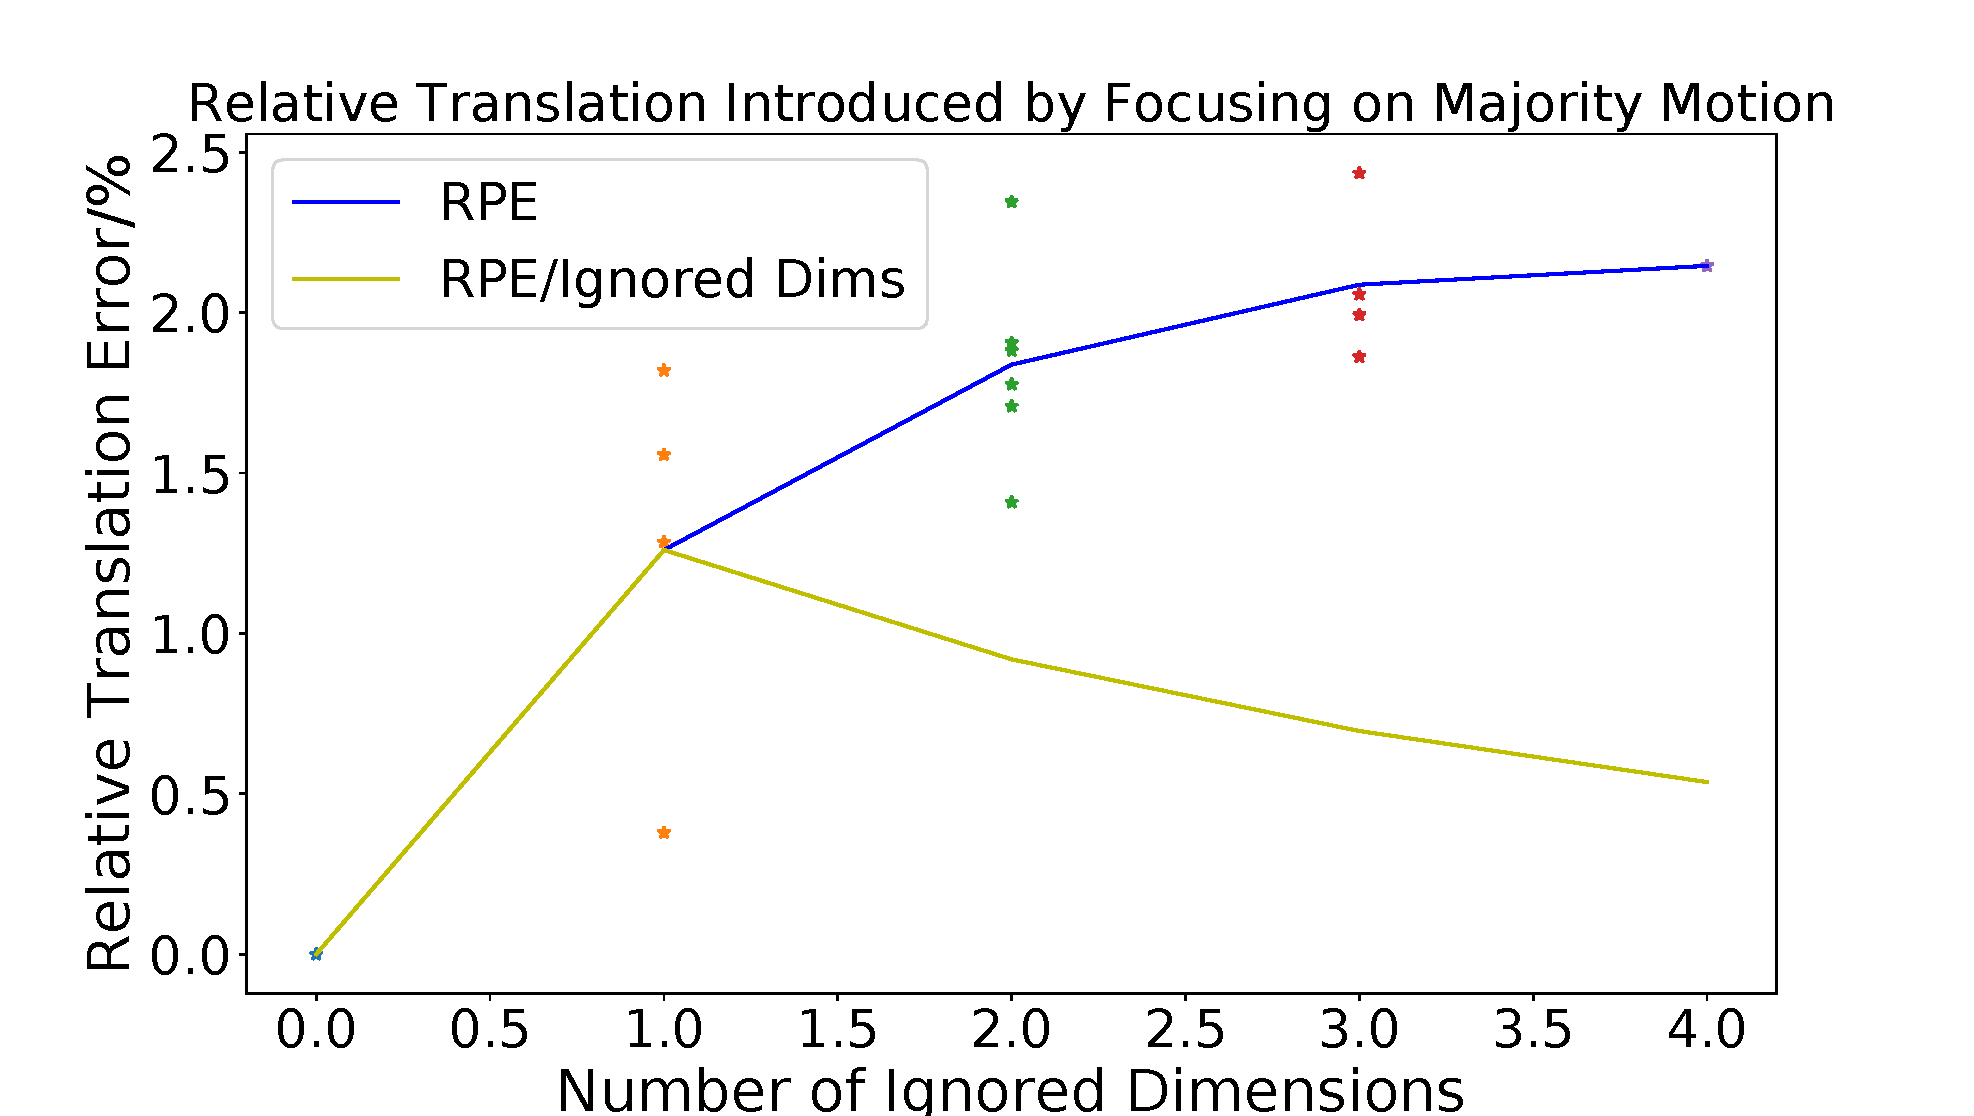
\includegraphics[width=0.9\textwidth]{datavo/info_loss.pdf}
    \caption{当忽略不同数量的维度时RPE平均值比较。}
    \label{fig:info_loss}
\end{figure}
在表\ref{tab:info_loss_1}中,列和行的名称分别代表保留的旋转轴和位移轴,NID表示忽略的维度数量。
当我们只保留z轴平移和y轴旋转时,忽略四个维度(NID=4)时,重建路径的RPE为2.20/%。我们将运动聚焦后的一些重构路径进行了可视化,如图\ref{fig:path_recon}所示,由此可以看出重构后的水平路径位移误差很小,误差在可接受范围。
位移主要积累在z轴上,z轴上的位移也受运行环境的影响,因为当路面有高低起伏时,位移会比较大(如图\ref{fig:conc_10}中表示的序列10),而当路面几乎平坦,位移就比较小(如图\ref{fig:conc_07}中的序列07)。更多可视化的重构路径详见附录。

\begin{figure}[ht]
    \centering
    \begin{subfigure}[b]{0.7\textwidth}
        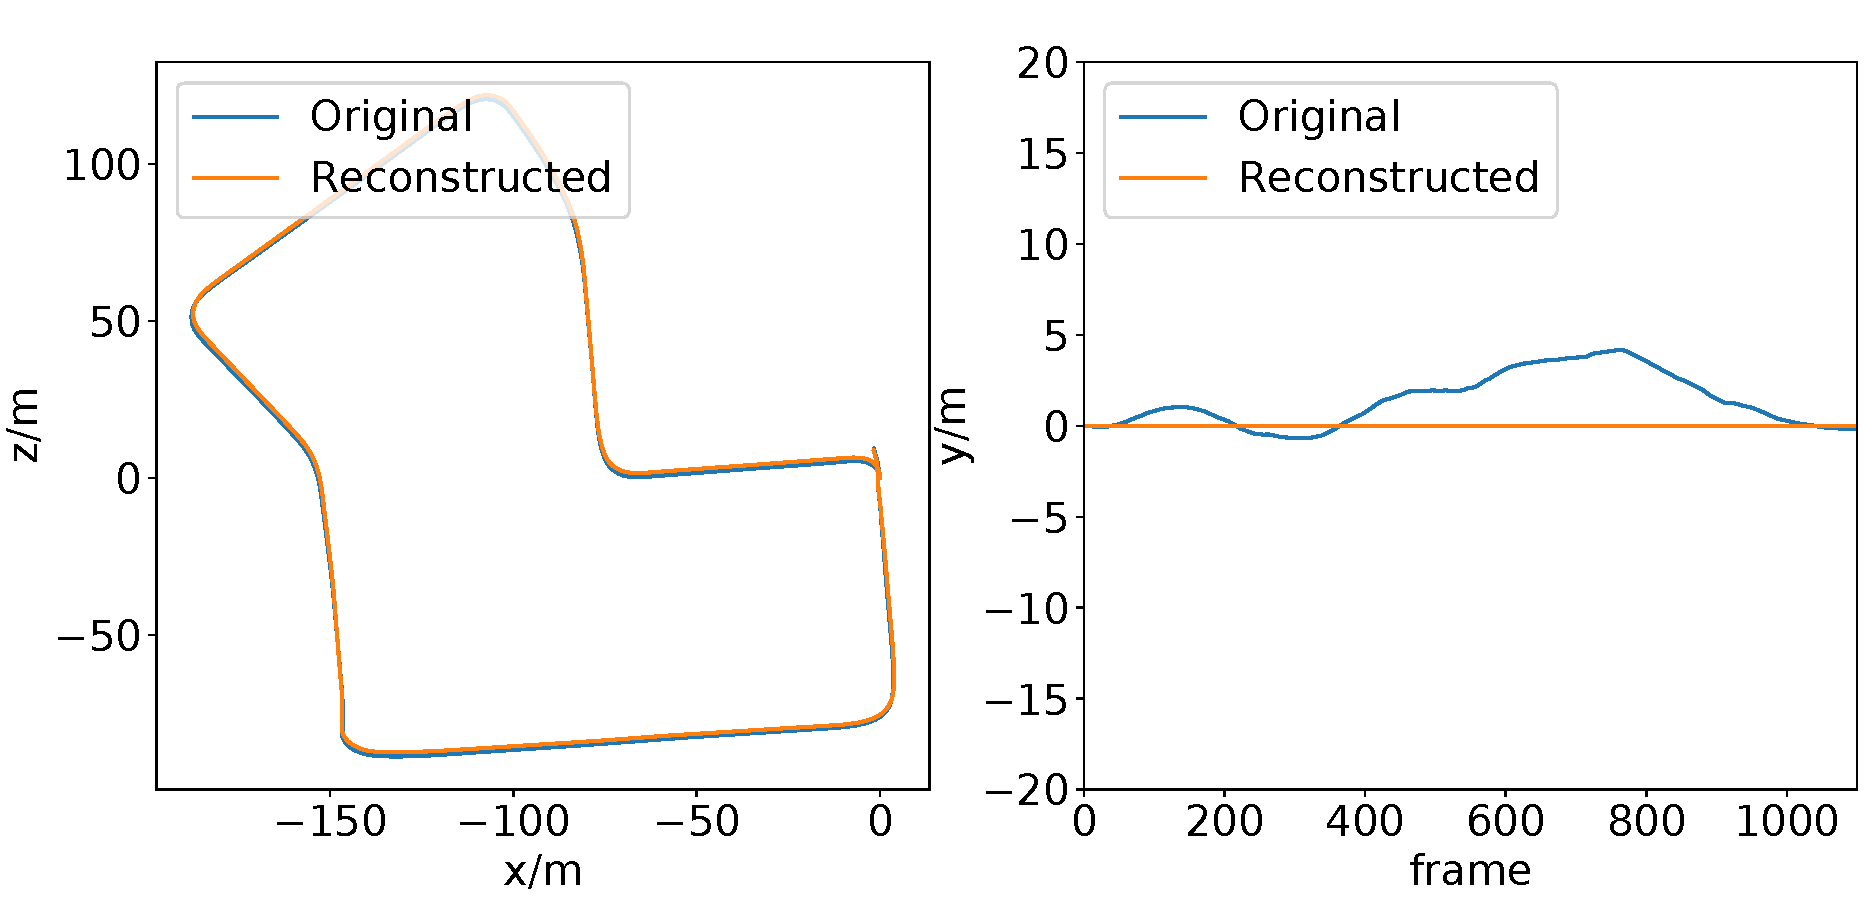
\includegraphics[width=\textwidth]{datavo/path_recon_07.pdf}
        \caption{}
        \label{fig:recon_07}
        \vspace{4pt}
    \end{subfigure}
    \begin{subfigure}[b]{0.7\textwidth}
        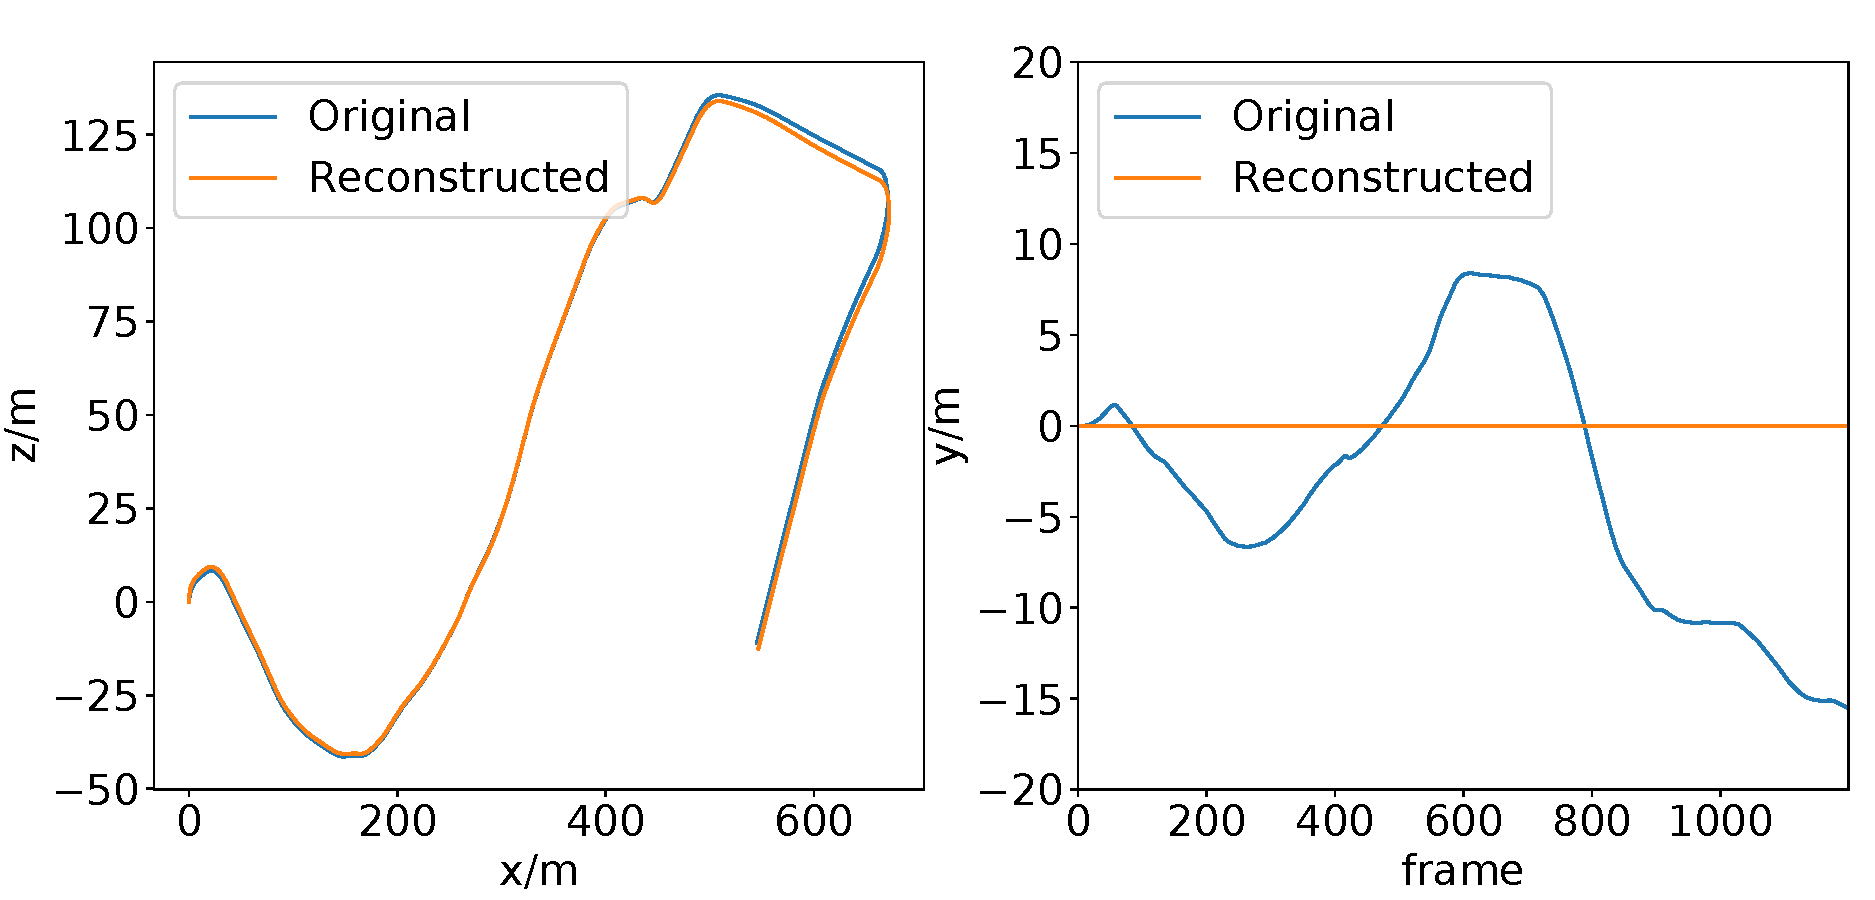
\includegraphics[width=\textwidth]{datavo/path_recon_10.pdf}
        \caption{}
        \label{fig:recon_10}
    \end{subfigure}
  \caption{重建路径的可视化。(a)重建的KITTI 07;(b)重建的KITTI 10。}     
  \label{fig:path_recon}
\end{figure}
为了更好的理解,我们还在图{RPEs}\ref{fig:info_loss}中可视化了RPE。 蓝色的线表示忽略不同维度数时的平均{RPEs}误差,我们将平均的
RPE(成本)除以所进行的维度数(收益),如图\ref{fig:info_loss}中的黄线所示,该比率可视为成本收益指标。只保留z轴平移和y轴旋转的成本收益比相对较小。
\subsubsection{Pose Displacement Improvement by Motion Decoupling}
\label{sec:info_decouple}
运动解耦的目标是减少忽略x轴平移时的姿势位移,其方法将在章节\ref{sec:motion_decouple}中介绍。
为了显示所提出的运动解耦的效率,我们定量评估了运动解耦所减少的姿态位移,如表\ref{tab:info_loss_1}所示。表中第一行表示当忽略X轴的平移时将导致更多的姿势偏移(从2.06%到2.20%)。
根据公式\eqref{eq:r_t_ratio},平移角$\alpha$和旋转角$\theta$之间是线性关系。然而,线性映射的斜率不是固定的,而是相对于不固定的前向运动$z$而言的。

为了简化问题,我们首先使用固定斜率参数来变换所有的前向运动,并使用不同比例测试RPE。结果如图所示\ref{fig:static_decouple}。当比值设为1.7时,我们得到的RPE最小。可以被解释为当车辆处于旋转状态时,车辆的平均前移距离约为$\frac{1.7-0.5}{l}$米。
为了更好地理解{图\ref{fig:static_decouple}中的}条形图,我们{使用}不同的颜色来表示不同的情形。运动解耦的目标是减少忽略x轴平移时的姿势位移,其方法将在章节\ref{sec:motion_decouple}中介绍。
为了显示所提出的运动解耦的效率,我们定量评估了运动解耦所减少的姿态位移,如表\ref{tab:info_loss_1}所示。表中第一行表示当忽略X轴的平移时将导致更多的姿势偏移(从2.06%到2.20%)。
根据公式\eqref{eq:r_t_ratio},平移角$\alpha$和旋转角$\theta$之间是线性关系。然而,线性映射的斜率不是固定的,而是相对于不固定的前向运动$z$而言的。
\begin{figure}[ht]
    \centering
    \begin{subfigure}[b]{0.45\textwidth}
        \centering
        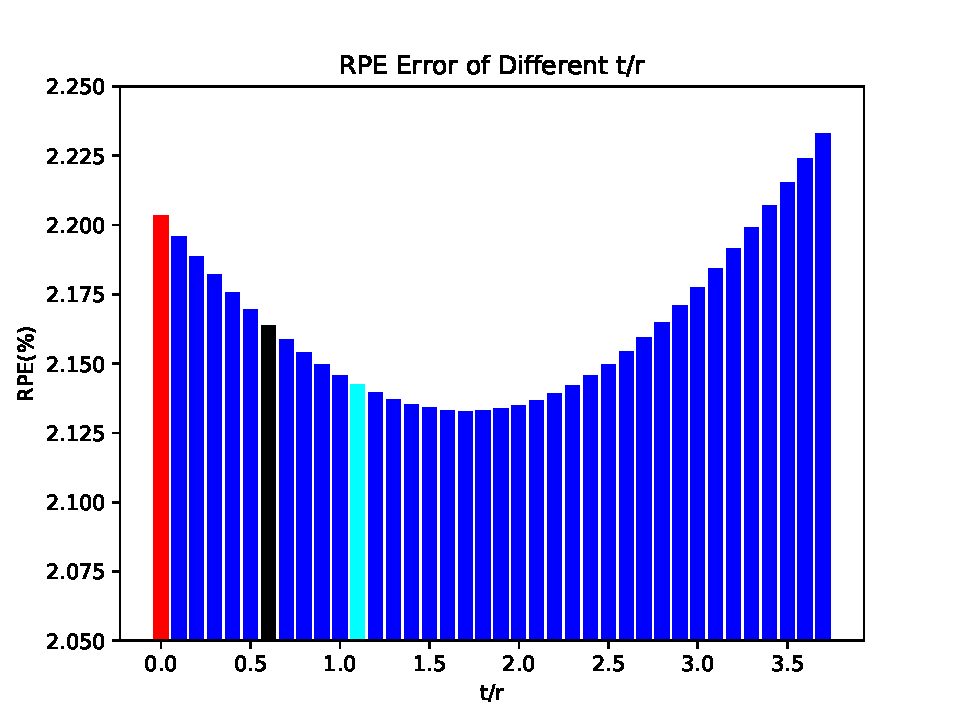
\includegraphics[width=0.9\textwidth]{datavo/r_t_ratio.pdf}
        \caption{}
        \label{fig:static_decouple}
    \end{subfigure}
    \begin{subfigure}[b]{0.45\textwidth}
        \centering
        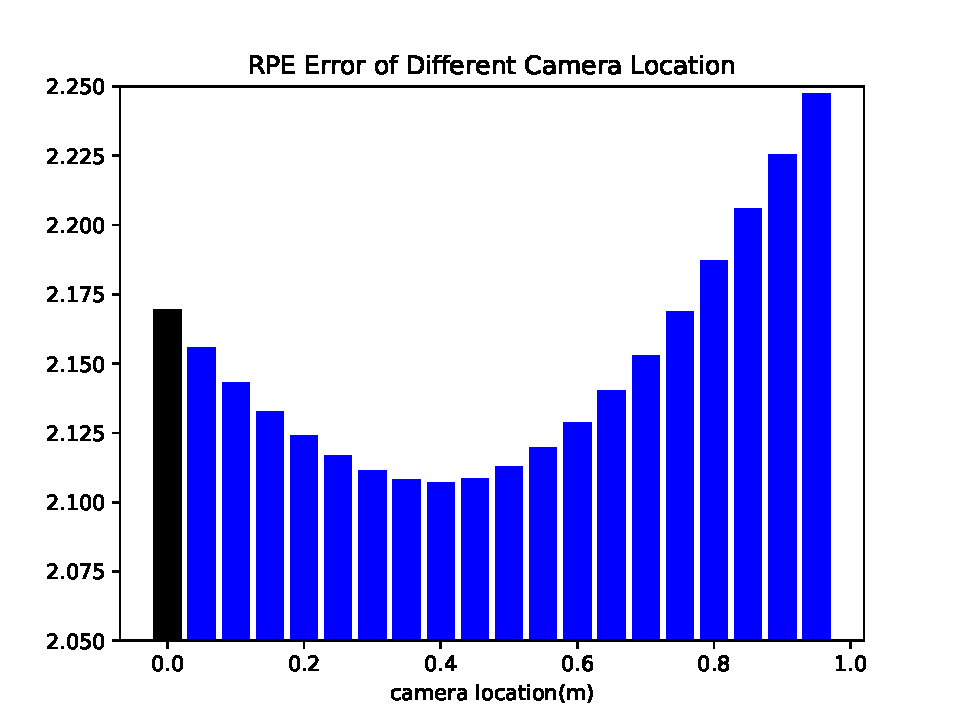
\includegraphics[width=0.9\textwidth]{datavo/r_t_ratio_2.pdf}
        \caption{}
        \label{fig:dynamic_decouple}
    \end{subfigure}
    \caption{Decoupling performance {visualization}. (a) Different fixed ratio; (b) Different dynamic ratio}.
    \label{fig:r_t_ratio}
\end{figure}


固定的比例会忽略车辆前行距离的影响,所以我们尝试使用动态比例。我们使用不同的摄像机位置$l$,用公式\eqref{eq:r_t_ratio}计算比率,然后评估重建路径的RPE,如图\ref{fig:dynamic_decouple}所示。
当摄像头位置设置为距离后轴0.4m时,RPE误差最小。
图\ref{fig:dynamic_decouple}中的黑色条形图代表着平移角$\alpha=0.5\theta$,这与图\ref{fig:static_decouple}中的黑色条形图相同。
计算比率时,用{\eqref{eq:r_t_ratio}计算,则评估重建路径RPE,如图\ref{fig:dynamic_decouple}所示。
当摄像头位置设置为距离后轴0.4m时,RPE误差最小。图\ref{fig:dynamic_decouple}中的黑条也代表着平移角$\alpha=0.5\theta$,这与图\ref{fig:static_decouple}中的黑条相同。
图\ref{fig:decouple}中可以直观地看到动态解耦和静态解耦的比较。{在图\ref{fig:decouple}中,蓝色条形代表没有运动解耦的RPE,黄色和绿色条形分别代表
静态解耦(比例设为1.7)和动态解耦(摄像机位置$l$设为0.4m)的RPE,红色条形代表我们同时保持x轴和z轴平移运动时的RPE}。
可以发现,动态解耦和静态{解耦}都可以降低RPE。当我们同时保持x轴平移和z轴平移时,动态{解耦}的RPE比静态{解耦}的RPE要低,而且更接近RPE。
\begin{figure}[ht]
    \centering
    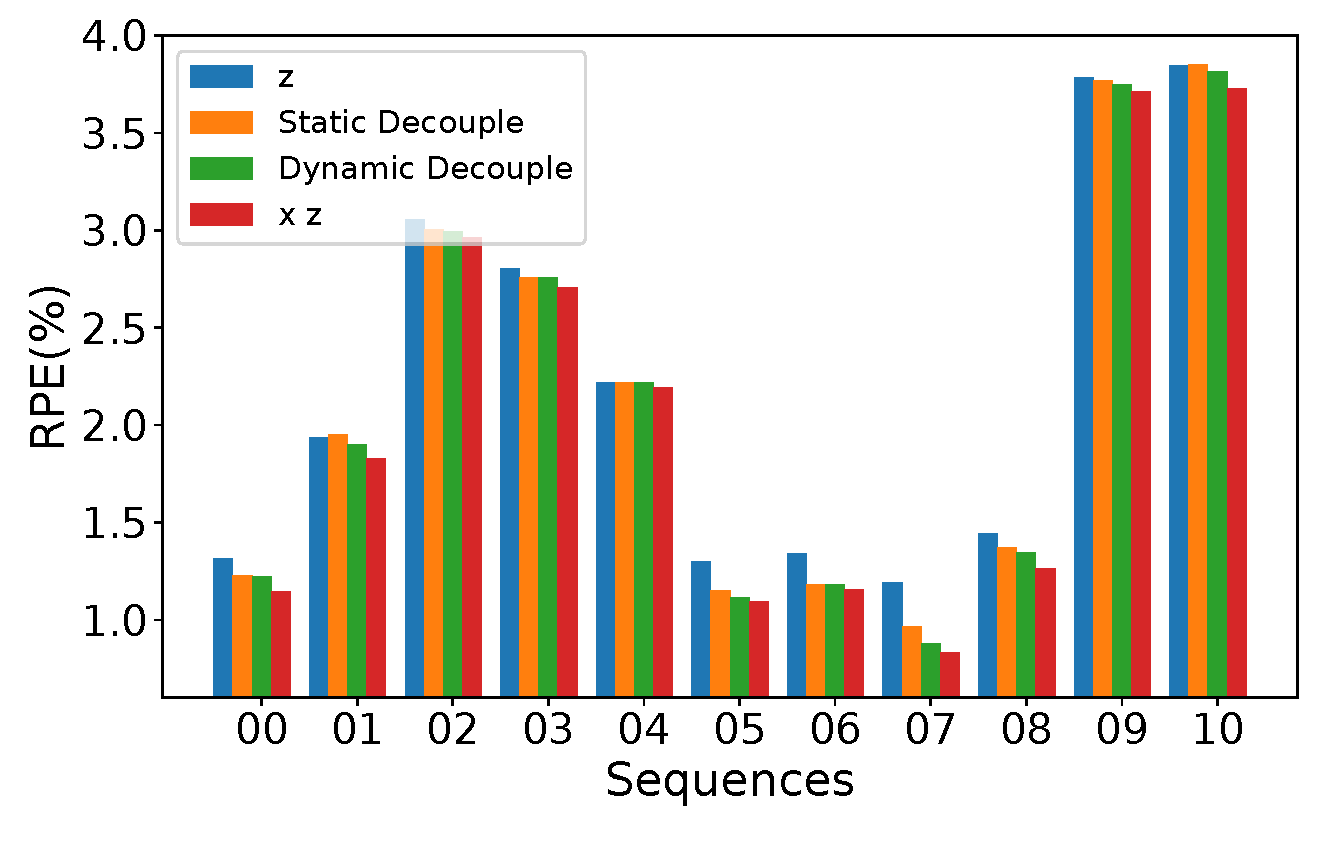
\includegraphics[width=0.6\textwidth]{datavo/decouple-crop.pdf}
    \caption{采用固定的解耦比率与动态比率时解耦性能比较。}
\end{figure}
\subsubsection{{Performance Improvement by Motion Focusing and Decoupling}}
\label{sec:ego_improvement}
\begin{table}[ht]
    \caption{The improvement of motion focusing}
    \label{tab:info_improve}
    \begin{center}
    \begin{tabular}{c c c c c c }
    \toprule
    % \hline
    \multirow{3}*{Train} & \multirow{3}*{Test} &\multicolumn{2}{c}{Learn All Motion} & \multicolumn{2}{c}{Learn $R_y, t_z$}\\
    & &Trans & Rot & Trans & Rot\\
    & & (\%) & (deg/m)  & (\%) & (deg/m)\\
    %  % \hline%\hline
    \midrule
     00 & 02 04 06 08 10 &26.8 & 0.137 & 23.9 & 0.110 \\
     00 02 & 04 06 08 10 &18.3 & 0.095 & 16.7 & 0.070 \\
     00 02 04 & 06 08 10 &17.6 & 0.091 & 16.9 & 0.076 \\
     00 02 04 06 & 08 10 &15.3 & 0.082 & 13.2 & 0.065   \\
    % \hline
    \bottomrule
    \end{tabular}
    \end{center}
 \end{table}

我们通过实验研究运动聚焦和解耦的影响。我们使用相同的训练数据来训练两种模型:
1)MFM(运动聚焦模型),只学习Y轴的旋转和Z轴的平移;2)AMM(全运动模型),学习六个自由度的运动。
在同一测试集上的RPE可以作为显示改进的指标。实验是在不同的训练-测试数据{分集}上进行的,以避免偶然性。我们记录了训练集的损耗变化曲线和测试集的{RPE}。
如图\ref{fig:training_loss}所示。对于所有的训练分割,MFM模型{收敛}比{AMM}模型快。
\begin{figure}[ht]
    \centering
    \begin{subfigure}[b]{0.45\textwidth}
        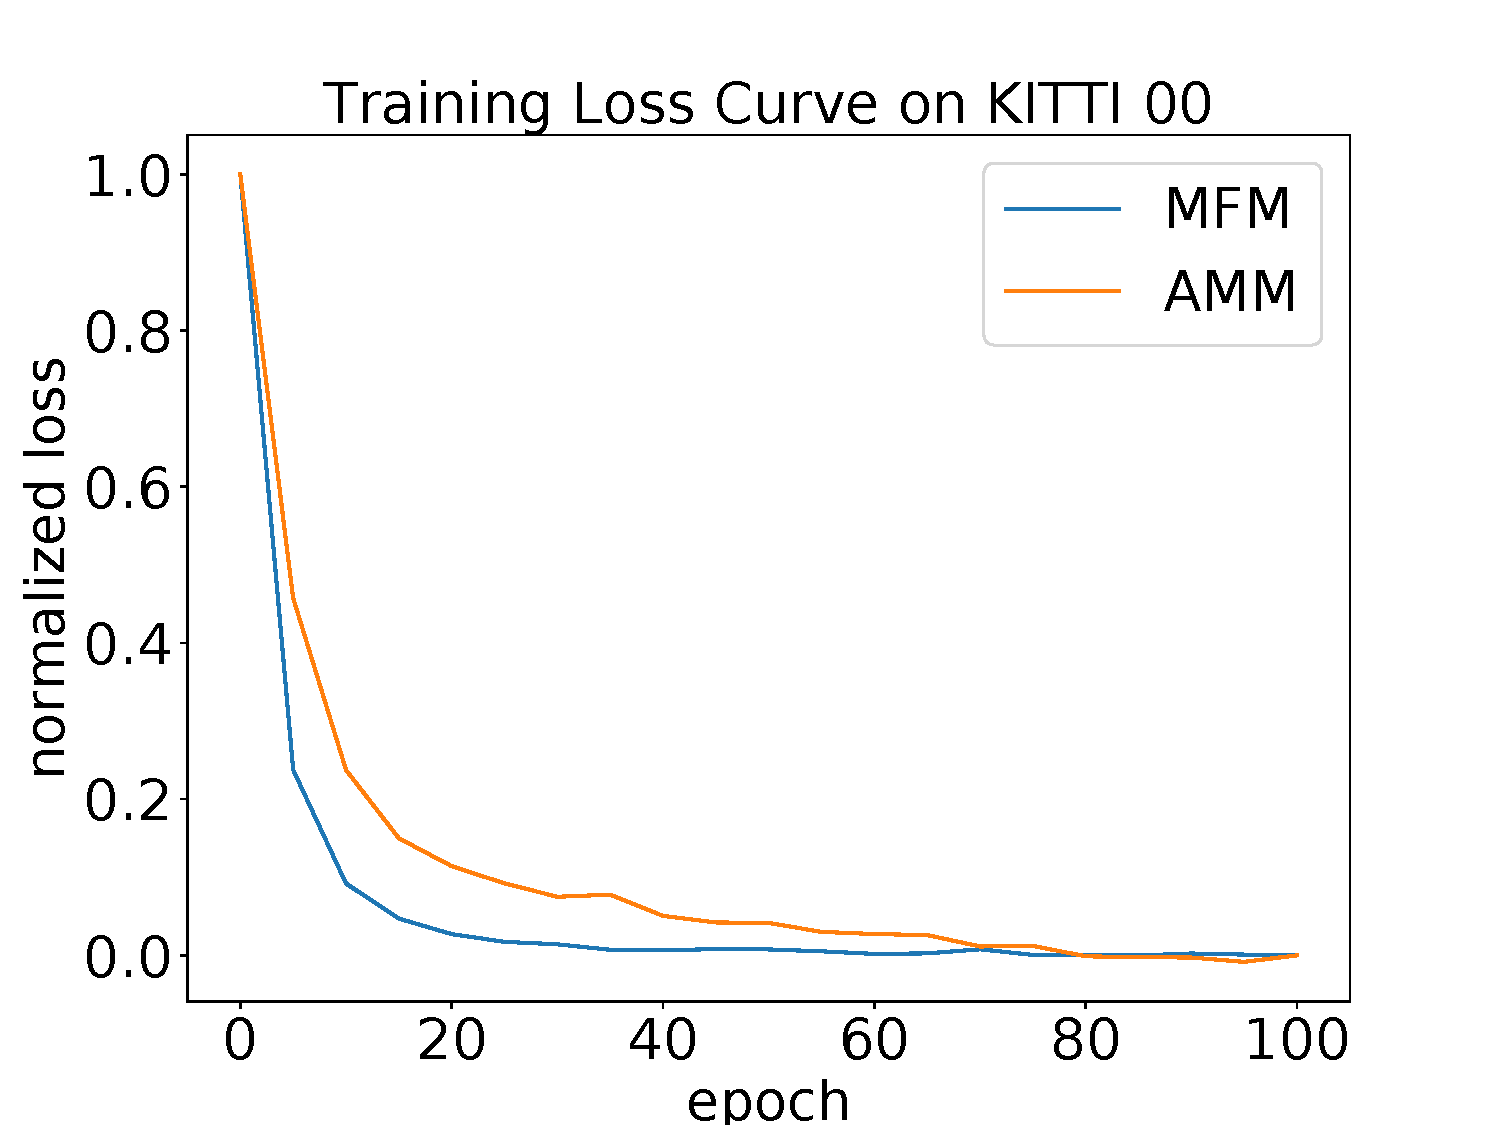
\includegraphics[width=\textwidth]{datavo/training_loss_0.pdf}
        \caption{}
        \label{fig:tl_0}
        \vspace{4pt}
    \end{subfigure}
    \begin{subfigure}[b]{0.45\textwidth}
        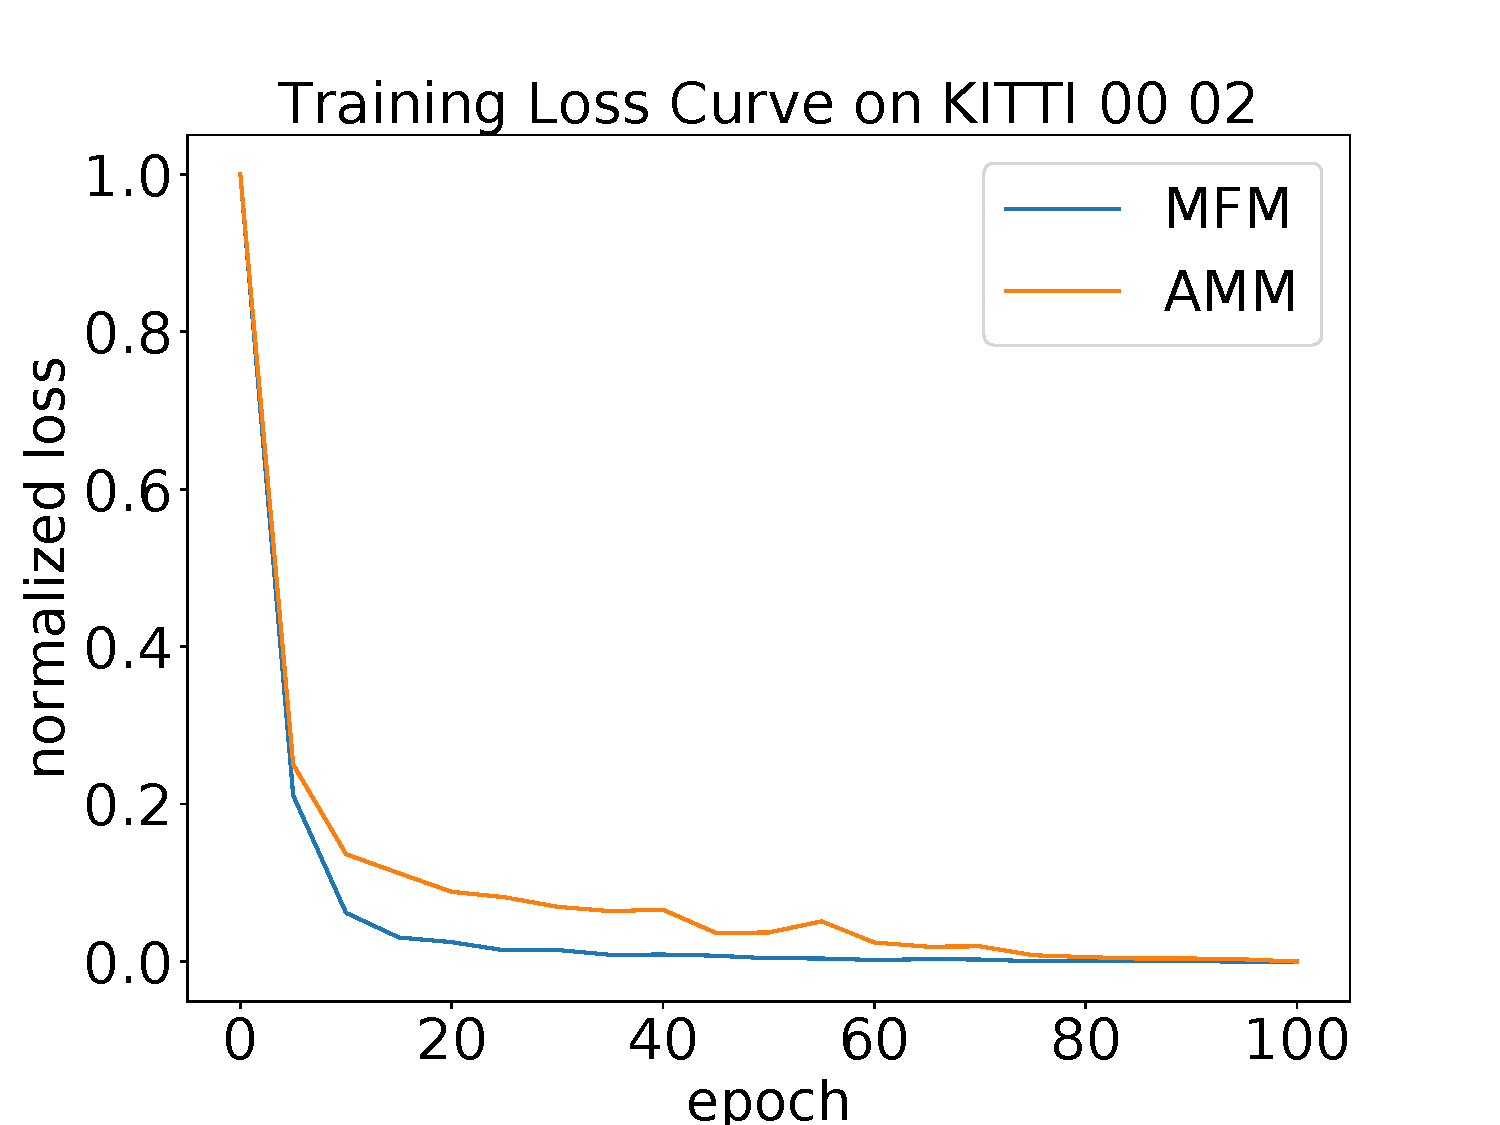
\includegraphics[width=\textwidth]{datavo/training_loss_0-2.pdf}
        \caption{}
        \label{fig:tl_02}
        \vspace{4pt}
    \end{subfigure}
    \begin{subfigure}[b]{0.45\textwidth}
        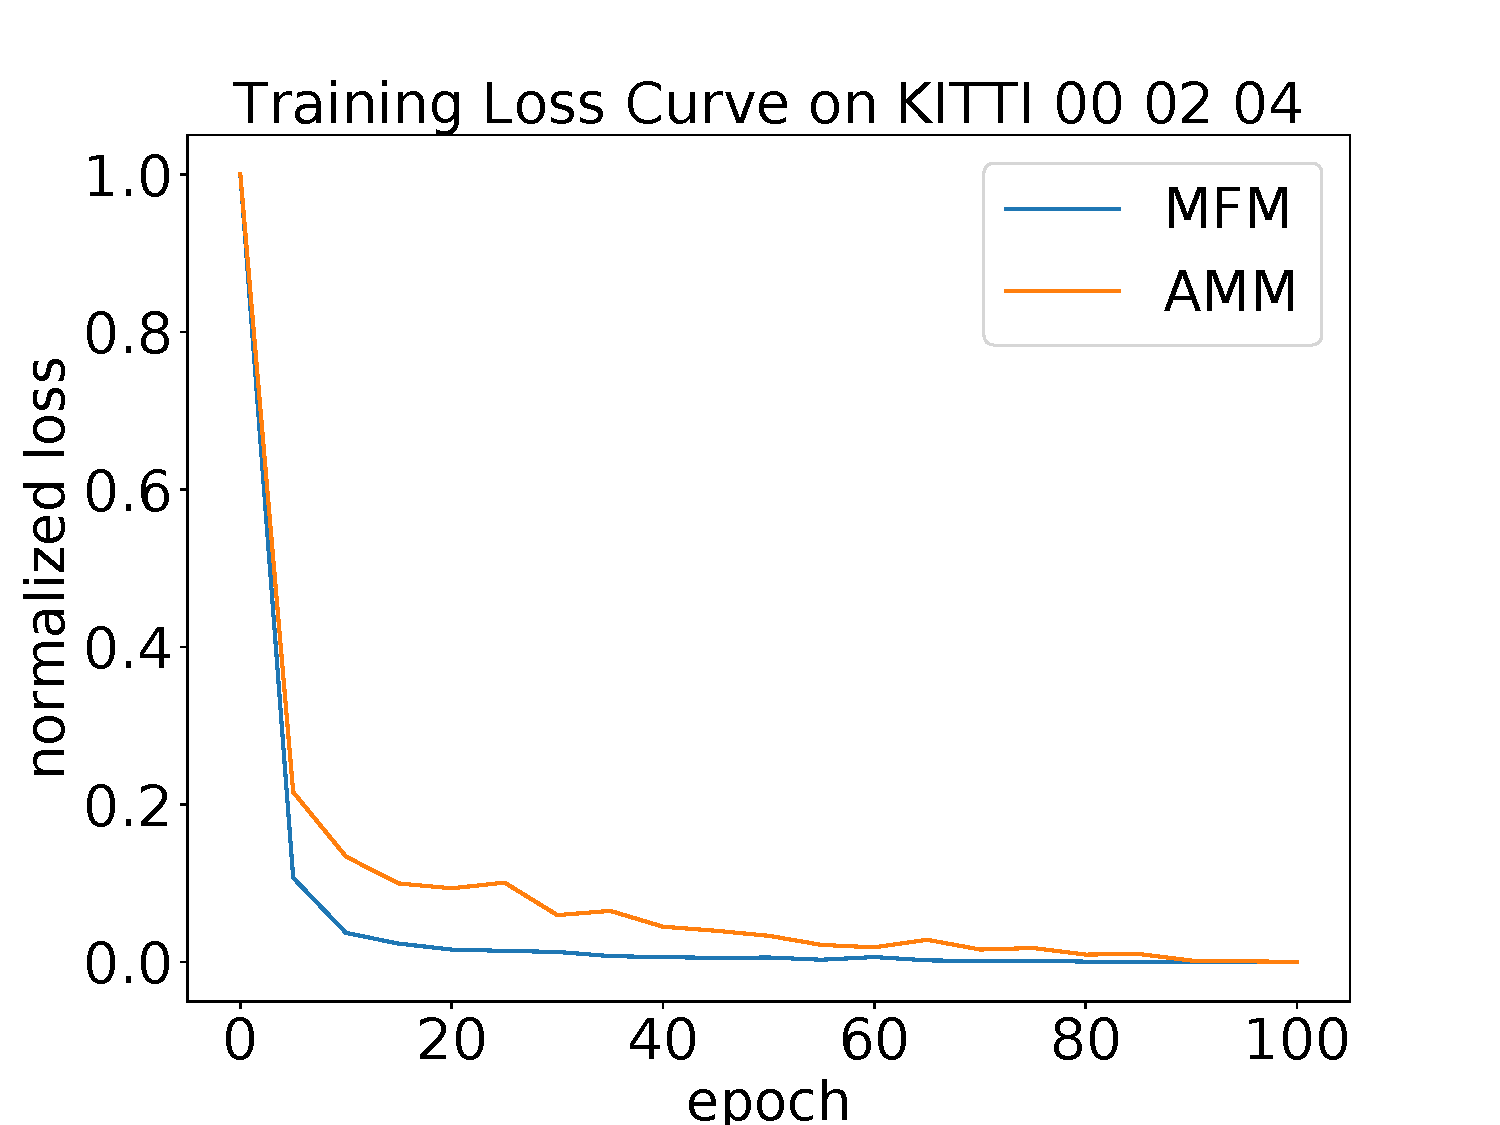
\includegraphics[width=\textwidth]{datavo/training_loss_0-4.pdf}
        \caption{}
        \label{fig:tl_024}
    \end{subfigure}
    \begin{subfigure}[b]{0.45\textwidth}
        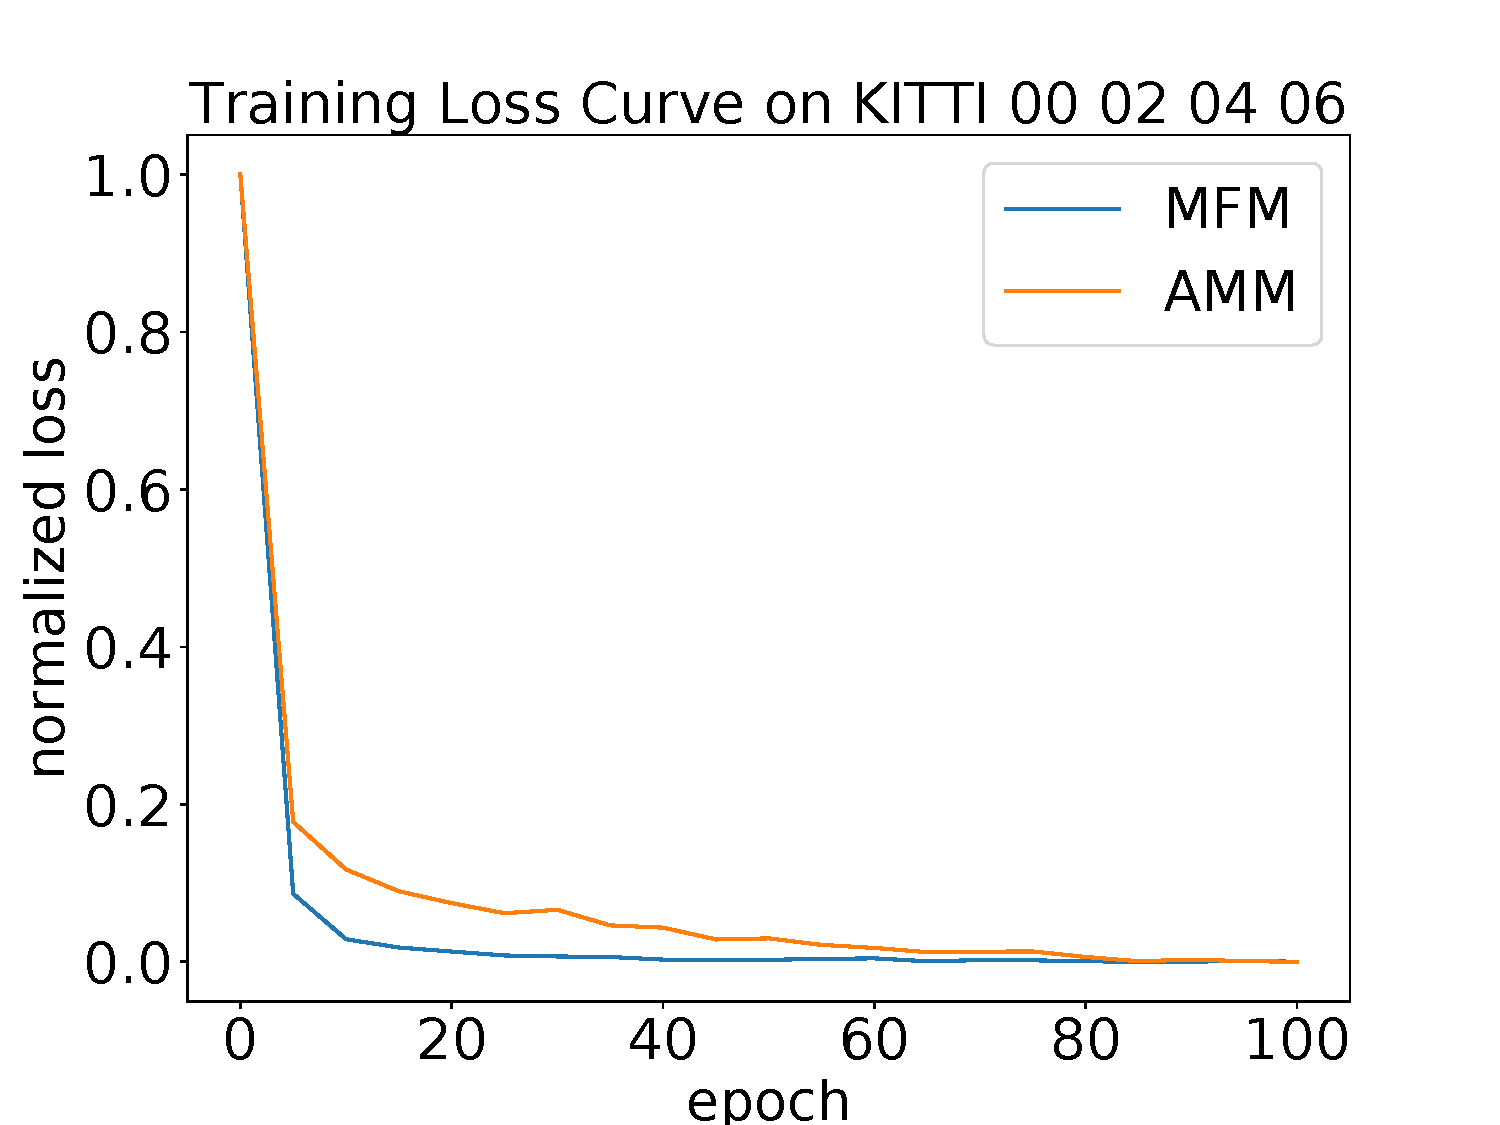
\includegraphics[width=\textwidth]{datavo/training_loss_0-6.pdf}
        \caption{}
        \label{fig:tl_0246}
    \end{subfigure}
\caption{训练损失曲线比较。(a) 在KITTI 00上的训练;(b) 在KITTI 00 02上的训练;(c) 在KITTI 00 02 04上的训练;(d) 在KITTI 00 02 04 06上的训练。}    
{\label{fig:training_loss}}
\end{figure}
\begin{figure}[h]
    \centering
    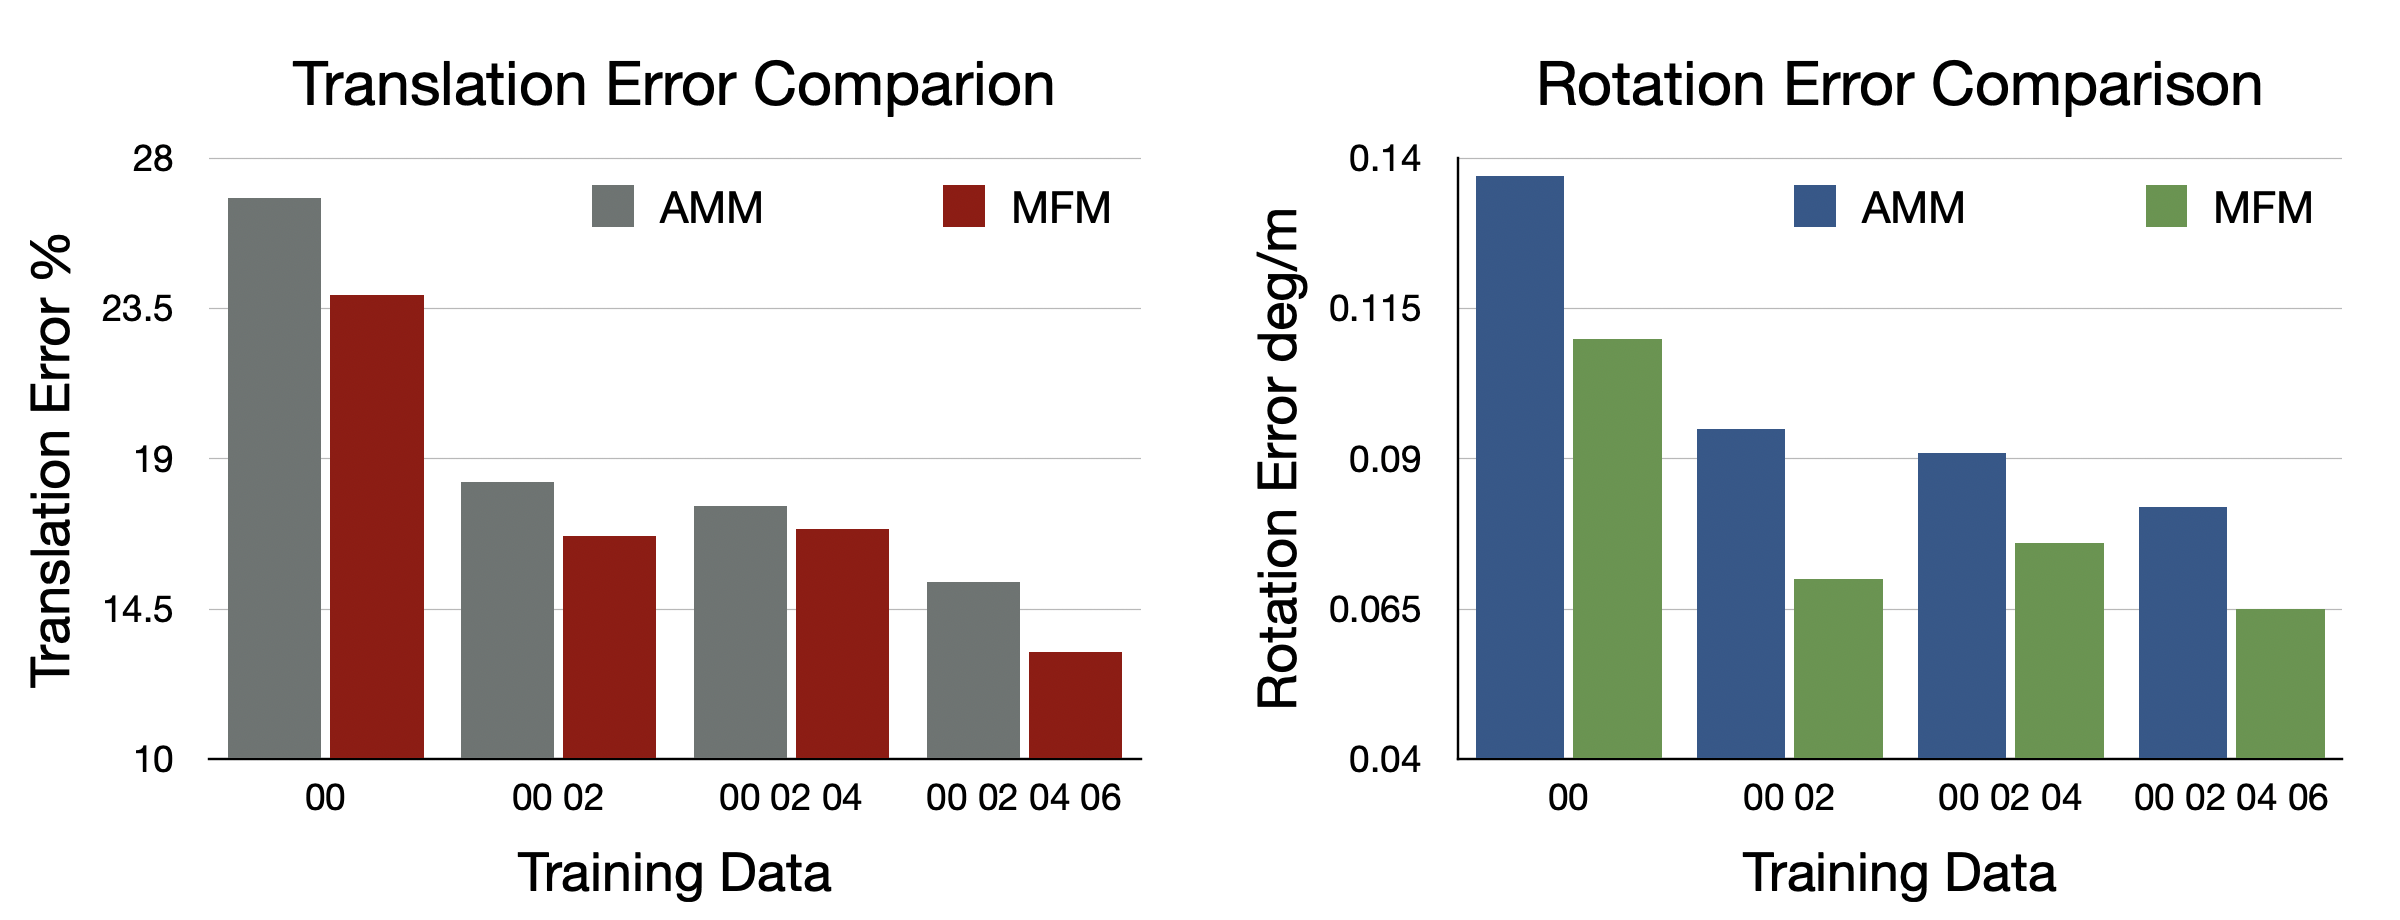
\includegraphics[width=0.8\textwidth]{datavo/focusing_train.png}
    \caption{聚焦训练后性能的提升。}
    \label{fig:focucing_train}
\end{figure}
不同训练模型的测试RPE记录在表\ref{tab:info_improve}中,并直观地显示在图\ref{fig:focucing_train}中。
我们可以发现,在不同的训练数据模式下,运动聚焦模型的结果都比学习所有6自由度的运动模型结果好,位移误差提高了约2\%,旋转提高了0.2degree/m。
从测试结果中还可以观察到,随着训练数据的增加,运动聚焦模型和所有运动模型的测试效果都越来越好。同时我们注意到,运动聚焦模型是由带有漂移姿势的地面真值{运动聚焦和解耦后}进行训练的,但测试性能仍然较好。

\subsubsection{与其他方法的比较}
\label{sec:compare}
\begin{table*}[!htbp]
    \caption{Comparison with other Learning-based Methods}
    \begin{center}
    \begin{tabular}{c c c c c c c c c c c c c c}
    \toprule
    % \hline
    \multirow{4}*{Seq} & \multicolumn{2}{c}{Zhan et al.} &\multicolumn{2}{c}{DeepVO} & \multicolumn{2}{c}{SfM-Learner.}& \multicolumn{2}{c}{GeoNet}&  \multicolumn{2}{c}{\multirow{2}*{Our Method }}\\
                       & \multicolumn{2}{c}{(from \cite{zhan2018unsupervised})}  & \multicolumn{2}{c}{(from \cite{wang2017deepvo})}&\multicolumn{2}{c}{(from \cite{zhou2017unsupervised})} &\multicolumn{2}{c}{(from \cite{yin2018geonet})} &\\
    %  % \hline%\hline
    \cline{2-3}  \cline{4-5}  \cline{6-7} \cline{8-9} \cline{10-11} \cline{12-13}
        & Trans & Rot  & Trans & Rot  & Trans & Rot &Trans & Rot& Trans & Rot\\ 
    & (\%) & (deg/m)  & (\%) & (deg/m)  & (\%) & (deg/m)& (\%) & (deg/m) & (\%) & (deg/m) \\
    \midrule
        09&11.92&0.0360&-&-&17.84&0.0678&26.93&0.0954&9.26&0.0229 \\
        10&12.62&0.0343&8.11&0.0883&37.91&0.1778&24.69&0.0843&9.10&0.0221 \\
    \midrule
    % \textbf{Avg.} & \textbf{84.0}\\
    Avg & 12.27 & 0.0351 &8.11 &0.0883  & 28.88 &0.1228 &25.81& 0.0899& 9.18&\textbf{0.0225}\\
    % \hline
    \bottomrule
    \end{tabular}
    \end{center}
    \label{tab:kitti_compare}
    \end{table*}
    
    \begin{table}[!htbp]
        \caption{Comparison with Popular Geometry-based Methods}
        \begin{center}
        \begin{tabular}{c c c c c c c c c c c c c c c c c c}
        \toprule
        % \hline
        \multirow{4}*{Seq} & \multicolumn{2}{c}{LIBVISO2} &  \multicolumn{2}{c}{ORBSLAM}& \multicolumn{2}{c}{\multirow{2}*{Our Method }}\\
                           &  \multicolumn{2}{c}{(from \cite{Song2015MoncularScale})}&\multicolumn{2}{c}{(from \cite{raul2015orb})}  &\\
        %  % \hline%\hline
        \cline{2-3}  \cline{4-5}  \cline{6-7} 
            & Trans & Rot  & Trans & Rot  & Trans & Rot\\ 
        & (\%) & (deg/m)  & (\%) & (deg/m)  & (\%) & (deg/m)& \\
        \midrule
            09&4.04& 0.0143&15.30&0.0026& 9.26&0.0229\\
            10&25.20 &0.0388&3.68&0.0048 &9.10&0.0221\\
        \midrule
        % \textbf{Avg.} & \textbf{84.0}\\
        Avg &14.62 & 0.0266& 9.49&0.0037 &\textbf{9.18}&0.0225\\
        % \hline
        \bottomrule
        \end{tabular}
        \end{center}
        \label{tab:kitti_compare_ge}
        \end{table}
    
我们将我们的算法与其他基于深度学习和{基于传统几何的}方法的算法进行比较。我们的模型在KITTI序列00-08上进行训练,在KITTI 09和10上进行测试,数据分割与其他基于卷积神经网络(CNN)方法相同
\cite{zhan2018unsupervised,zhou2017unsupervised,yin2018geonet}。测试的RPE记录在表\ref{tab:kitti_compare}和\ref{tab:kitti_compare_ge}中。
由于SfM-Learner \cite{zhou2017unsupervised}和GeoNet \cite{yin2018geonet}的模型都是以自监督的方式进行无绝对尺度的训练,因此在评价前,它们的路径与地面路径真值是一致的。Zhan等人的模型\cite{zhan2018unsupervised}、DeepVO\cite{wang2017deepvo}和我们的方法都是用绝对尺度训练的,所以不需要对齐。单目模式的ORB-SLAM\cite{raul2015orb}和LIBVISO\cite{Geiger2011IV}的尺度也是与地面真实路径对齐的。

如表\ref{tab:kitti_compare}所示,我们的方法优于其他基于(自我运动模型主要由卷积层构建的)CNN的方法\cite{zhan2018unsupervised,zhou2017unsupervised,yin2018geonet},并与基于CNN-RNN{(RNN是Recurrent Neural Network的缩写)}的方法\cite{wang2017deepvo}竞争,后者可以利用时间信息优化姿势。

与两种效果较好的主流传统方法LIBVISO单目法(LIBVISO monocular \cite{Geiger2011IV})和ORB-SLAM单目法(ORB-SLAM monocular \cite{raul2015orb})比较,我们得到了较好的平均位移性能。


\subsection{Discussion}

在本节中,我们将对结果进行总结,对性能进行分析,并说明所提出的方法的局限性。
\subsubsection{The Efficiency of the Proposed Method}

从上面的实验结果来看,可以得出四个方面的结论。
1)运动聚焦不会带来太大额外的位姿偏移。平均RPE只有2\%左右,也就是说{车辆姿态}跑了100米后会有2米左右的漂移。路径可视化显示,重建后的路径是可以接受的。
2)运动解耦可以减少姿势位移。运动解耦利用y轴旋转和x轴平移的相关性来降低重构的姿势位移偏移。动态解耦的性能优于静态解耦。
对于动态解耦,需要对摄像机的位置有所要求。在上述实验中,摄像头位置是根据地面真实数据计算出来的。在实际操作中,如果训练数据是自己采集的,也可以直接测量得到。
3)运动聚焦{和解耦}可以从两个方面提高自我运动估计性能。首先,它{缩短了训练时间,所有的训练实验都在20个epoch内收敛,但所有运动的模型在大约60个epoch后才收敛,所以运动聚焦模型与所有运动模型相比,可以减少大约2/3的训练时间。另外,尽管运动聚焦和运动解耦后训练的地面真值姿势有一定的漂移,但{MFM}的测试性能比{AMM}更好。
4)在与基于几何的方法比较的过程中,发现基于几何的方法并不稳健,在不同序列上获得的性能各异。我们的方法更加稳定和稳健,平均性能更好。我们的方法也优于其他基于CNN的方法,在与利用RNN提高性能的DeepVO\cite{wang2017deepvo}比较时,我们也获得了更好的相对旋转性能,但位移性能比DeepVO差。


\subsubsection{Why Motion Focusing { and Decoupling} Works}

运动聚焦{和解耦}性能较好的原因有三点:首先,地面车辆的运动是受约束的,且分布不均衡,忽略不明显的运动不可能造成太大的姿态{位移}误差,这一点已在第\ref{sec:info_loss}节中得到证明。而这也是运动聚焦的根本基础};第二,不重要的运动太有限,没有足够的信噪比,所以模型在瞄准它们建模时,很容易被噪声干扰;第三,当我们只聚焦于二维运动时,训练任务变得{简单很多}。当采用{轻型}模型时,训练数据相对丰富。
实验证明,增加训练数据量确实能提高测试性能,如表\ref{tab:info_improve}所示。

\subsubsection{The Limitation} 

当汽车有近似{平面}运动时,所提出的方法可以获得更好的性能。
当有明显的{x轴旋转时,性能将下降。}如图\ref{fig:decouple}所示,序列09和10的RPE误差相对较高,因为在{这}两个序列中,地面车辆的运动不是{平面}的,如图\ref{fig:path_recon}所示。为了解决这个局限性,一个可行的方法是采用其他传感器,如IMU(惯性测量单元)来估计X轴的旋转,这可以作为所提出的模型所估计的平面运动的补充。

此外,{另一个限制是}因为我们的算法是基于摄像机是平放且是向前看的假设,所以如果摄像机有俯仰角,那么车辆的向前运动将被映射成Z轴运动和Y轴运动。如果摄像机有一个俯仰角,那么车辆的向前运动将被映射成Z轴运动和Y轴运动。在这种情况下,摄像机俯仰角$\sigma$应在训练前进行校准。然后,平移运动应该被重新定义为
\begin{equation}
    t_\sigma = \begin{pmatrix} 1 & 0 & 0 \\ 0 & \cos(\sigma) & -\sin(\sigma)\\ 0 & \sin(\sigma) & \cos(\sigma) \end{pmatrix} t
    \label{eq:pitch_correction}
\end{equation}

这些局限性也可以通过利用视觉里程测量的多模型结构来解决,每个子模型只关注地面车辆的一个维度运动,六自由度可以用六个分离的模型来学习,在这种情况下,应该分析模型权重分摊的影响。
\section{本章小结}
\label{sec:conclusion}
本文通过提出运动聚焦和运动解耦,将地面车辆的运动聚焦为两个自由度上的运动。实验证明了运动聚焦的可行性,并通过定量的姿态位移评估,进一步降低了姿态位移。基于地面车辆的旋转模型,我们提出了运动解耦,进一步降低了姿势位移。我们构建了一个轻型CNNs网络模型来模拟二自由度运动,它可以在CPU上实时运行。实验证明,运动聚焦和解耦可以提高小我运动估计性能,缩短收敛时间。在KITTI数据集上与其他方法的比较表明,所提出的方法的性能与其他端到端的视觉里程测量方法相当,甚至更好,并且比基于几何的方法更稳健。

